\documentclass[a4paper,10pt]{book}
\usepackage[utf8]{inputenc}
\usepackage{Matematica}



\addbibresource{Matematica.bib}
\begin{document}

  \tableofcontents
	
  \chapter{Presentazione}
bla bla
  \chapter{Introduzione}

\section{Introduzione, Introduction}		
Mathematics è il tentativo di raccolta di appunti e materiale per studiare con profitto nei corsi di laurea in Matematica.

Il programma di riferimento \`{e}, principalmente, quello dell'Universit\`{a}
di Bologna, anche se, non essendo iscritto a nessuno corso, ho cercato di integrare i programmi (syllabus) con i corsi di altre Universit\'{a}. Diciamo che la matematica \'{e} tale.
Comunque, nel confrontare i vari corsi proposti dalle varie universit\'{a} mi sono accorto che argomenti trattati in geometria vengano trattati in altri corsi denominati algebra lineare oppure, geometria e algebra.

Pertanto, mi sono preso la libert\'{a} di organizzare tutti i concetti di tutte le materie in un unico corpo. Questo punto non \`{e} banale perch\'{e} apre alcune questioni oggi
approfondite in corsi quali \textit{Interazione persona-computer}, \textit{Semantic web}, \textit{Intelligenza artificiale}, \textit{Logica}, \textit{Machine learning}, \textit{Mathematical Knowledge Management}, etc.

Il materiale raccolto \'{e} ancora in fase embrionale. 


\section*{Nota}
Il materiale contenuto nella cartella di google drive è ad accesso limitato. Per accedere cliccare sul link seguente e seguire le istruzioni per ottenere
l'accesso alla cartella. \url{https://drive.google.com/drive/folders/0Bx2fZ0r5vhSSSDdvWkVjNG9YQjQ}

\section*{Introduzione}
I libri che trovate nella \href{https://drive.google.com/drive/folders/0Bx2fZ0r5vhSSSDdvWkVjNG9YQjQ}{folder}, sono stati raccolti seguendo la bibliografia proposta dai Docenti di Università
italiane e straniere. Si trovano i classici di algebra, analisi, geometria, etc. Inoltre, ho selezionato alcuni libri perchè hanno una data stampa risalenete al massimo
agli ultimi tre anni che in genere sono fatti bene perchè raccolgono le esperienze maturate studiando i testi che li hanno preceduti.

Oltre a libri, troverete dispense, papers, etc. Al momento non ho fatto distinzione tra libri o altro pdf ma ho semplicemente suddiviso il materiale seguendo
più o meno le materie indicate nel \href{Syllabus.html}{Syllabus} e quindi troverete le seguenti cartelle: Algebra, Analisi, Topologia, Geometria, etc.

\section*{Come utilizzare il materiale pdf}
Esistono buoni articoli che ci danno una panoramica su come utilizzare un libro di testo o una dispensa. Alcuni professori, specie nelle lezioni introduttive, danno
informazioni riguardanti lo studio della materia nel suo complesso e con esso anche un accenno sull'utilizzo dei libri di testo.


  
  \part{Mathematical logic and foundations}
  \chapter{Mathematical logic and foundations}

%\chapter{Introduzione ai fondamenti della Matematica}

Vi sarete di certo chiesti: \textit{ho letto questa dimostrazione per la decima volta e ancora non ci capisco nulla, perch\'e?}, \'e lecito chidersi perch\'e dopo tutto la dimostrazione di qualsivoglia teorema non la devo mica inventare, la vorrei
semplicemente leggere come in un libro di cucina. In questo viene in aiuto lo studio dei fondamenti della matematica, chiamata da Hilber metamatematica.
 
Metamathematics is the study of the tools or techniques needed by an undergraduate student in order to be able to study mathematics profitably. 

E, di fatto, Hilbert, essendo un matematico, la sa lunga sull'uso delle parole per definire gli oggetti. La metamatematica è lo studio della matematica con l'utilizzo della stessa matematica. Probabilmente il termine moderno di metamatematica \'e \textit{logica matematica}.

Bene, una volta che abbiamo imparato che cos'\'e la metamatematica ovvero abbiamo acquisito una serie di strumenti della logica matematica possiamo iniziare a studiare matematica, e perch\'e non iniziare dalla teoria degli insiemi.

La teoria ingenua degli insiemi è un modello matematico che si pone alla base di tutta la matematica.  
Putroppo successivamente si scoprirono dei bug ovvero
il modello portava a dei paradossi e quindi fu aggiustata da Zermelo, Fraenkel e Skolem (ZFS). 

Ecco il modello ingenuo:  
Un insieme è una collezione di elementi distinti con due particolarità:  
\begin{itemize}
 \item gli elementi dell'insieme possono essere, a loro volta, insiemi.
 \item esiste un insieme composto da nessun insieme, detto insieme vuoto.
\end{itemize}




\section{Derivata}
Il calcolo differenziale nasce soprattutto per affrontare problemi di geometria, in particolare quello delle tangenti.




\chapter*{PREFAZIONE}
Il lavoro che segue non \'{e} la ristampa di un trattato precedente dello stesso autore, intitolato \textit{L'analisi matematica della logica}. Le sue prime parti sono, \'{e} vero,
dedicate allo stesso argomento, e il libro incomincia stabilendo il medesimo sistema di leggi fondamentali, ma i suoi metodi sono pi\'{u} generali e il campo delle sue applicazioni
\'{e} di gran lunga pi\'{u} ampio. Il libro espone i risultati, maturati in anni di studio e di riflessione, di un principio d'indagine relativo alle operazioni dell'intelletto, la cui
prima esposizione fu stesa in poche settimane da che fu concepita l'idea.

\textbf{Questo e il secondo lavoro di boole ma e da considerare quello principale. Per fare un analogia struts... Bisogna prima di leggere questo trattato
  leggere altri due trattati che erano le basi per poter leggere il libro di Boole nel 1850.  
  \textit{Elementi di logica} dell'arcivescovo Whately oppure \textit{Lineamenti delle leggi del pensiero} del signor Thomson.
}

\chapter{Natura e scopo dell'opera}

\section{}
Scopo di questo trattato \'{e} d'indagare le leggi fondamentali di quelle operazioni della mente per mezzo delle quali si attua il ragionamento; di dar loro espressione nel linguaggio
simbolico di un calcolo e d'istituire, su questo fondamento, la scienza della logica costruendone il metodo; di fare, di questo stesso metodo, la base di un metodo generale per
l'applicazione della dottrina matematica della probabilit\'{a} e, in ultimo, di ricavare dai diversi elementi di verit\'{a} portati alla luce nel corso di queste indagini alcune
indicazioni probabili sulla natura e la costituzione della mente umana.

\section{}
Non c'\'{e} quasi bisogno di ricordare che questo progetto non \'{e} del tutto originale, e tutti sanno che i filosofi hanno dedicato una parte considerevole della loro attenzione
a quelle che sono, dal punto di vista pratico, le sue suddivisioni principali: la logica e la teoria della probabilit\'{a}. Nella forma che le fu data dagli antichi e dagli Scolastici,
la logica \'{e} quasi esclusivamente associata al grande nome di Aristotele: e fino ai giorni nostri, salvo alcuni cambiamenti inessenziali, \'{e} rimasta praticamente tal quale fu
presentata all'antica Grecia nelle disquisizioni in parte tecniche e in parte metafisiche dell'\textit{Organon}. Dal canto suo, l'indirizzo della ricerca originale si \'{e} orientato
principalmente verso questioni di filosofia generale le quali, pur essendo sorte fra le dispute dei logici, sono andate oltre quello che erano all'origine, dando alle epoche successive
della speculazione la loro inclinazione e il loro carattere particolari. Le et\'{a} di Porfirio e Proclo, di Anselmo e Abelardo, di Ramus e Descartes, conclusesi con la contestazione
di Bacone e Locke, stanno davanti alla nostra mente come esempi delle pi\'{u} remote influenze che questo studio ha esercitato sul cammino del pensiero umano: in parte perch\'{e} hanno
suggerito fecondi argomenti di discussione, in parte perch\'{e} hanno dato luogo alle critiche contro le sue pretese illegittime. Dall'altra parte, la storia della teoria della
probabilit\'{a} \'{e} stata contraddistinta in misura molto maggiore da quel costante sviluppo che costituisce la caratteristica propria della scienza. Il genio precoce di Pascal alle origini
di questa disciplina, le pi\'{u} profonde tra le speculazioni matematiche di Laplace nelle sue fasi pi\'{u} mature (e qui non faccio menzione di altri nomi, non meno noti di questi)
furono impegnati nel perfezionamento di questa teoria. Como lo studio della logica ha esercitato la propria influenza sul pensiero per le questioni di metafisica, ad esso affini,
cui ha dato occasione, cos\'{i} quello della teoria della probabilit\'{a} deve ritenersi importante per lo sviluppo che ha impresso alle parti pi\'{u} astratte della scienza matematica.
Si \'{e} inoltre ritenuto giustamente che ciascuna di queste discipline avesse di mira, oltre che fini pratici, anche fini teorici. L'oggetto della logica, infatti, non \'{e} solo
quello di metterci in grado di trarre inferenze corrette da premesse date, n\'{e} l'unica pretesa della teoria della probabilit\'{a} \'{e} quella di insegnarci come fondare su solide
basi il mestiere di assicuratore sulla vita o di raccogliere in formule i dati significativi delle innumerevoli osservazioni che si compiono in astronomia, in fisica, o in quel campo delle ricerche
sociali che oggi va rapidamente acquistando importanza. Entrambi questi studi presentano anche un interesse di altro genere, derivante dalla luce che gettano sui poteri dell'intelletto.
C'insegnano in qual modo il linguaggio e il numero servano da strumento e da ausilio ai processi del ragionamento; ci rivelano, in certa misura, la connessione esistente fra i diversi
poteri del nostro comune intelletto; mettono davanti a noi, nei due domin\^{i} della conoscenza dimostrativa e di quella probabile, i modelli essenziali della verit\'{a} e della
correttezza: modelli che non sono stati ricavati dall'esterno, ma sono profondamente radicati nella costituzione delle facolt\'{a} dell'uomo. Questi fini speculativi non cedono n\'{e}
in dignit\'{a}, n\'{e}, si potrebbe aggiungere, in importanza, agli scopi pratici con il perseguimento dei quali sono stati spesso associati nel corso della loro storia. Lo svelare le
leggi e le relazioni pi\'{u} nascoste di quelle facolt\'{a} superiori del pensiero grazie alle quali giungiamo a possedere, o portiamo a compimento, tutto ci\'{o} che va oltre la pura
e semplice conoscenza percettiva del mondo e di noi stessi, \'{e} un fine la cui dignit\'{a} non ha certo bisogno di essere raccomandata a uno spirito raziocinante.

\chapter{Dei segni in generale e dei segni adatti alla scienza della logica in particolare; delle leggi alle quali \'{e} sottoposta quest'ultima classe di segni}



\section{DEFINIZIONE}
Aristotelian or traditional logic is a “subject-predicate” logic and is therefore concerned only with a portion of the sum total of logical truth.

It confines itself to the four forms of categorical proposition 
known as the A, E, I, and O forms.

In the second place, it treats subalternation as a valid form of inference. 
That is, it assigns (tacitly at least) conventional meanings, different from those employed in modern 
(i.e. symbolic or mathematical) logic, to the four categorical forms, meanings such that subalternation holds.

These two characteristics, however, are not sufficient to define Aristotelian logic. 
For an indefinite number of systems could be devised which possess these two properties. 
Since further distinguishing traits of Aristotelian logic will appear only in the course of our investigation, 
a definition of Aristotelian logic framed in terms of its essential properties cannot be given at the outset.


\section{DEFINIZIONE}
Constructive mathematics is distinguished from its traditional counterpart, classical mathematics, 
by the strict interpretation of the phrase “there exists” as “we can construct”. 
In order to work constructively, we need to re-interpret not only the existential quantifier but all the logical connectives and quantifiers as instructions on how to construct 
a proof of the statement involving these logical expressions. 


\section{DEFINIZIONE}
Intuitionistic logic, sometimes more generally called constructive logic, refers to systems of symbolic logic that differ from the systems used for classical logic 
by more closely mirroring the notion of constructive proof. 
In particular, systems of intuitionistic logic do not include the law of the excluded middle and double negation elimination, 
which are fundamental inference rules in classical logic. \cite{k1}

Intuitionistic logic encompasses the principles of logical reasoning which were used by L. E. J. Brouwer in developing his intuitionistic mathematics, 
beginning in [1907]. Because these principles also underly Russian recursive analysis and the constructive analysis of E. Bishop and his followers, 
intuitionistic logic may be considered the logical basis of constructive mathematics. 



\section{Elementi di logica dell'arcivescovo Whately}


\subsection{DEFINIZIONE}
Gli \textit{Elementi di logica} del 1853 dell'arcivescovo Whately era il testo che Boole consiglia di leggere prima di leggere il suo trattato del 1954.


\section{DEFINIZIONE}
Dato un insieme numerabile di simboli \'{e} possibile trovare, per ogni formula, un algoritmo che mi dica se quella formula \'{e} o no derivabile dall'insieme di simboli e dalle regole date.


\section{DEFINIZIONE (1)}
An interpretation is an assignment of meaning to the symbols of a formal language.  

assignment = ???  
symbol = ???  
formal language = ???

\section{DEFINIZIONE (2)}
An interpretation $I$ is a function which assigns to any atomic formula $p_i$ a truth value

\[
I(p_i) \in {0,1}
\]

If $I(p_i)=1$ then $p_i$ is called true under the interpretation $I$  
If $I(p_i)=0$ then $p_i$ is called false under the interpretation $I$

\section{DEFINIZIONE (2)}
An interpretation $A$ is a structure





\section{Introduzione - Axiom of extensionality}
Dovrebbe essere abbastanza evidente che, l'uguaglianza tra due strutture matematiche, \'{e} un fatto "quasi" arbitrario e quindi in un certo senso devo definire che cosa si intende
per uguaglianza tra due insiemi. Ebbene, Zermelo identifica tale concetto di uguaglianza con il concetto di estenzionalit\'{a}, cio\'{e} di estensione. Dietro questo assiome
c\'{e} dell'altro. In un certo senso, si potrebbe dire che \'{e} il meccanismo del contare all'interno della teoria degli insiemi. Quindi dall'assioma non ricavo "quanti" sono
gli elementi dei due insiemi ma sono certo del fatto che i due insiemi contengono lo "stesso numero" di elementi.

\section{NOTAZIONE}
\[
  \forall A \forall B (\forall X (X \in A \Leftrightarrow X \in B ) \Rightarrow A = B)
\]




\section{Passaggio da linguaggio naturale a linguaggio simbolico (linguaggio formale?)}
\subsection{ESEMPI}
%If $x$ is an ancestor of $y$ is an ancestor of $z$, then $x$ is an ancestor of $z$. $P(x,y) \and P(y,z) \to P(x,z)$



\section{Logica e Fondamenti}


\section{Introduction}
La logica si divide in logica dei predicati e logica delle proposizioni. La logica dei predicati è la logica delle proposizioni con l'aggiunta dei quantificatori
per ogni ($\forall$) ed esiste ($\exists$). Quando si passa alla logica dei predicati sembra che le proposizioni vengano rappresentate come delle funzioni. 

\section{Syllabus}
\begin{itemize}
 \item Notion
 \item Symbol
 \item Variable (symbol)
 \item Language
 \item Reasoning
 \item Magnitude
 \item Law of excluded middle
 \item Propositional function
 \item \href{Appartenenza.html}{Appartenenza}
 \item Inclusione
 \item Uguaglianza (tra insiemi)
 \item \href{TeoriaIngenuaInsiemi.html}{Teoria ingenua degli insiemi}
 \item Cantor = teoria dei numeri e teoria (ingenua) degli insiemi
 \item \href{./Esistenza.html}{Esistenza}
 \item \href{./Transfinito.html}{Transfinito}
 \item Coerenza
 \item Indipendenza
 \item \href{./SviluppiDecimali.html}{Sviluppi decimali}
 \item Funziona caratteristica di un sottoinsieme.
 \item Rappresentazione posizionale dei numeri
 \item \href{./Interpretation.html}{Interpretation}
 \item \href{./Passaggio.html}{Passaggio da linguaggio naturale a linguaggio simbolico (linguaggio formale?)}
 \item \href{ClassicalLogic.html}{Classical Logic}
 \item \href{FormalLogic.html}{Formal Logic}
 \item \href{./IntuitiveLogic.html}{Intuitive Logic}
 \item Constructive Logic
 \item \href{ConstructiveMathematics.html}{Constructive Mathematics}
 \item Symbolic Logic
 \item \href{Entscheidungsproblem.html}{Entscheidungsproblem}
 \item \href{./RecursiveFunctionTheory.html}{Recursive Function Theory}
\end{itemize}



\section{Temi d'esame}
  \begin{itemize}
   \item 1
  \end{itemize}

\section{Dispense di partenza}
\begin{itemize}
  \item Dispense Prof. Placci Unibo
  \item \url{http://www.settheory.net/}
  \item \url{http://www.mafy.lut.fi/study/LogicAndDiscreteMethods/Lectures/Lecture2.pdf}
  \item \url{http://cse.unl.edu/~choueiry/F07-235/files/PredicatesQuantifiers.pdf}
  \item \url{http://cgi.csc.liv.ac.uk/~frank/teaching/comp118/lecture2.pdf}
  \item \url{http://emilkirkegaard.dk/en/wp-content/uploads/0415400678.Routledge.Logic_.An_.Introduction.Dec_.2005.pdf}
\end{itemize}

\section{GOOGLE SEARCHES}
\begin{itemize}
 \item predicate logic solved examples
\end{itemize}

\section{Altre pagine latex da integrare in questi appunti}
\begin{itemize}
 \item \url{https://github.com/baudo2048/appunti}
\end{itemize}





\chapter{Semiotica}
Multirappresentazione
%\chapter{Fondamenti di logica matematica e teoria degli insiemi}
La logica matematica (o metamatematica), sia dal punto di vista dell'apprendimento che della matematica pura, la chiave di volta per decifrare i segni usati in matematica.

La teoria degli insiemi \`e, invece, il linguaggio con il quale la logica matematica viene rappresentata.

\section{Logica, Storia e Filosofia}
\begin{itemize}
 \item \href{HowToStudy.pdf}{How to study mathematics}
  \item \href{Metamathematics.pdf}{Metamathematics}
  \item \href{Logics.pdf}{Logica}
  \item \href{QuantumTheory.pdf}{Quantum Theory}
  \item \href{history.pdf}{History} 
\end{itemize}

\section{Set Theory}
\subsection*{Basics}
\begin{itemize}
 \item Insieme, famiglia, classe, collezione.
 \item Appartenenza
 \item Unione tra insiemi
 \item Intersezione tra insiemi 
 \item inf e sup di un insieme
 \item Significato di $A - B$ dove $A$ e $B$ sono insiemi.
 \item Complementary
 \item Well-ordering
 \item Zermelo: proof that every set can be well-ordered
\end{itemize}
 
\subsection*{Assiomi della teoria degli insiemi}
\begin{itemize}
 \item \href{./Extensionality.pdf}{Axiom of extensionality}
 \item \href{./EmptySet.pdf}{Axiom of empty set}
 \item Axiom of pairing
 \item Axiom of union
 \item Axiom of infinity
 \item Axiom of power set
 \item Axiom of regularity
 \item Axiom schema of specification
 \item Axiom of choice
\end{itemize}

\subsection*{Funzioni, applicazioni, mappe, operazioni, relazioni}
\begin{itemize}
 \item \href{CartesianProduct.pdf}{Cartesian product}
 \item \href{Relation.pdf}{Relation between sets}
 \item \href{EquivalenceRelation.pdf}{Equivalence relation}
 \item \href{OrdinamentoInsieme.pdf}{Ordinamento di un insieme (lemma di Zorn)}
 \item \href{Function.pdf}{Funzione}
 \item Applicazione
 \item Mappa
 \item \href{Operazione.pdf}{Operazione}
 \item Operazione di somma tra numeri
 \item Operazione di somma tra vettori
 \item Operazione di somma tra matrici
 \item \href{./FunzioneSuriettiva.pdf}{Funzione suriettiva (o surgettiva, o suriezione)}
 \item Funzione iniettiva
 \item Funzione bigettiva
 \item Cardinality (of a group for example)
\end{itemize}

\subsection*{Teoria delle Funzioni}
\begin{itemize}
 \item Dominio di una funzione
 \item Maggiorante di una funzione
 \item Minorante di una funzione
 \item Estremo superiore di una funzione
 \item \href{FunzioneMassimoMinimo.pdf}{Massimo e minimo di una funzione}
\end{itemize}

\section{Assiomi di Peano}
\begin{itemize}
 \item 
\end{itemize}

\section{Church's Postulates}
\begin{itemize}
 \item 
\end{itemize}

\section{Hilbert's Axioms}
\begin{itemize}
 \item 
\end{itemize}





%\chapter{Foundations of Arithmetic - Frege}
%\chapter{Formal Logic}

\section{DEFINIZIONE}
Formal logic e symbolic logic sono la stessa cosa. Aristotele per esempio, non usava simboli per studiare la logica formale.

\section{NOTAZIONE}

\section{ESEMPIO}

\begin{thebibliography}{100}
  \bibitem{k1} \url{https://www.britannica.com/topic/formal-logic}
  \bibitem{k2} \url{https://math.stackexchange.com/questions/1812585/what-is-the-difference-between-symbolic-and-formal-logic}
\end{thebibliography}


%\chapter{Esistenza}

\section{DEFINIZIONE}
La definizione che cerco non \'{e} quella relativa al concetto di quantificatore esistenziale ma quella relativa all'esistenza di un oggetto matematico.
Quando un oggetto matematico si può dire che esiste?
%\chapter{EmptySet}

\section{DEFINIZIONE}

\section{NOTAZIONE}
\[
  \exists X \forall Y \neg (Y \in X)
\]
\section{ESEMPIO}



%
\section{DEFINIZIONE}
Che va al di l\'{a} del finito.

\section{NOTE}
Transfinito dunque è sinonimo del termine infinito che si usa oggi in matematica, anche se secondo me il termine transfinito è qualcosa di più ampio
nel senso che l'infinito è un transfinito perch\'{e} va oltre il finito ma transfinito potrebbe anche essere qualcos'altro.

Per quanto riguarda la logica matematica il problema \'{e} capire qual'\'{e} la dimostrazione della sua esistenza e della sua coerenza.


  
  \part{Combinatorics}
  \chapter{Combinatorics}

\chapter{Permutations, words, matrices}

\begin{definizione}
Sia $X$ un insieme non vuoto. Si dice permutazione su $X$ ogni applicazione bigettiva di $X$ in se stesso.
\end{definizione}

In generale, per indicare una permutazione si usano le lettere greche minuscole, es. $\sigma$, e la cosiddetta notazione matriciale,
nella quale sono riportarte (nella seconda riga) le immagini secondo $\sigma$ degli elementi di $X$ (scritti nella prima riga):
\[
\left(
 \begin{array}{cccc}
  1 & 2 & ... & n \\
  \sigma(1) & \sigma(2) & ... & \sigma(n)
 \end{array}
\right)
\] 

\begin{definizione}[Permutazione identica - elemento neutro rispetto alla composizione di permutazioni]
In questa notazione, l'applicazione identica corrisponde ad una matrice con due righe uguali:
\[
\left(
 \begin{array}{cccc}
  1 & 2 & ... & n \\
  1 & 2 & ... & n \\
 \end{array}
\right)
\]
\end{definizione}

Indicheremo tale applicazione (detta permutazione identica), più semplicemente, con il simbolo $id$. 

\begin{definizione}[Inversa di una permutazione]
per ottenere l’inversa di una permutazione basta scambiare la prima e la seconda riga e riordinare la prima. 
\end{definizione}

\begin{definizione}[Insieme delle permutazioni]
Denoteremo con $S(X)$ l'insieme delle permutazioni su $X$. 
\end{definizione}

Il numero di elementi di $S(X)$ è uguale a $n!$, dove $n$ è il numero di elementi dell'insieme $X$.

\begin{definizione}[Ciclo di una permutazione (1)]
Per \textit{ciclo di una permutazione} si intende il nome della notazione utilizzata per rappresentare una permutazione.
\end{definizione}

\begin{definizione}[Ciclo di una permutazione (2)]
Sia $n$ un intero positivo. Si dice \textit{ciclo (o permutazione ciclica)} ogni $\sigma \in S_n$ per cui esistono un intero
positivo $l$ e $a_1, ..., a_l \in \{1, ..., n\}$ a due a due distinti tali che
\begin{itemize}
 \item $\sigma(a_1)=a_2, \sigma(a_2)=a_3, ..., \sigma(a_l)=a_1$;
 \item $\sigma(k)=k$ per ogni $k \in \{1, ..., n\} \setminus \{a_1, ..., a_l\}$.
\end{itemize}
\end{definizione}

Il numero $l$ si dice lunghezza di $\sigma$. Una permutazione ciclica di lunghezza $l$ si dice anche l-ciclo.

\begin{definizione}[Ciclo di una permutazione (2)]
Sia $r$ un intero positivo, $2 \leq r \leq n $ e siano dati $r$ elementi distinti $i_1, i_2, ..., i_r \in X=\{1,2,...,n\}$.
Col simbolo $\gamma = (i_1 i_2 ... i_r)$ si denoti la permutazione $\gamma \in S_n$ tale che:
\begin{enumerate}
 \item $\gamma (i_k) = i_k$ se $i_k \notin \{i_1, i_2, ..., i_r\}$
 \item $\gamma(i_k)=i_{k+1}$ se $1 \leq k \leq r-1$
 \item $\gamma (i_r)=i_1$
\end{enumerate}
\end{definizione}
Tale permutazione è detta ciclo di lunghezza $r$.
Se il ciclo ha lunghezza 2 viene detto trasposizione o scambio.

Il solo ciclo di lunghezza 1 è la permutazione identica.

Il ciclo di lunghezza 2 è detto trasposizione o scambio.

La scrittura ciclica di un l-ciclo non è unica. Se $l>1$, il ciclo ammette esattamente $l$ scritture cicliche distinte,
ottenute tramite rotazioni successive degli indici verso sinistra.

Un ciclio è una lista di indici fra parentesi, e conveniamo che rappresenti la permutazione che associa a ogni indice nel ciclo
quello successivo.

\medskip
Ad esempio, il ciclo
\[
 (12345)
\]
rappresenta la permutazione che manda 1 in 2, 2 in 3 e così via fino a 5 in 1. Due cicli sono disgiunti se non hanno lettere in comune.
Per esempio, (123) e (45) sono disgiunti, ma (123) e (124) no. 

\section{Composizione di permutazioni = Prodotto di cicli}
Per scrivere la composizione di permutazioni rappresentate da cicli,
basta scrivere i cicli di seguito.

Non è difficile calcolare la permutazione risultante da una composizione di cicli: basta, per ogni lettera, "seguire il suo destino" lungo
i vari cicli. Per esempio,
\[
 (123)(135)(24) = \left(\begin{array}{ccccc}
                         1 & 2 & 3 & 4 & 5 \\
                         4 & 5 & 3 & 2 & 1 Cicli\\
                        \end{array} \right)
\]
Come abbiamo fatto il conto? Cominciamo da 1: il primo ciclo manda 1 in 2, il secondo non tocca il 2, il terzo manda 2 in 4: concludiamo
che i tre cicli mandano 1 in 4. Il primo ciclo manda 2 in 3, il secondo 3 in 5, e il terzo non tocca 5: concludiamo che i tre cicli
mandano 2 in 5, e così via. Notate che alla fine del conto c'è un controllo di coerenza molto semplice:  tutti i numeri
nella seconda riga devono essere distinti.

\begin{definizione}[Decomposizione di una permutazione in cicli]
Decomporre una permutazione in cicli disgiunti vuol dire rappresentarla sotto forma di cicli.
\end{definizione}

Come fare a ottenere una rappresentazione in cicli di una permutazione? Basta "seguire" una lettera qualunque fino a trovare
un ciclo: per esempio, in 
\[
\left( \begin{array}{cccc} 1 & 2 & 3 & 4 \\ 3 & 1 & 2 & 4 \\ \end{array} \right) 
\]
abbiamo che 1 va in 3, 3 va in 2 e 2 va in 1; quindi il primo ciclo che troviamo è (123). A questo punto non ci rimane che 4,
che però va in sé, e formerebbe un ciclo di lunghezza 1. I cicli di lunghezza 1 per convenzione non si scrivono, e
quindi la permutazione si scrive (123).

NB: Secondo me se segui questo procedimento per forza di cose devi trovare cicli disgiunti.

\begin{definizione}[Periodo di una permutazione]
Data una qualsiasi permutazione, il suo periodo sarà il minimo comune multiplo dei periodi dei cicli disgiunti in cui essa si decompone. 
\end{definizione}

INTRODUZIONE: \\
Ogni permutazione di $S_n$, $n>2$, è prodotto di trasposizioni. Osserviamo però che tali trasposizioni possono non essere
disgiunte ed inoltre la rappresentazione di una permutazione como prodotto di trasposizioni non è unica. Ad esempio, la permutazione
$\alpha=(123)$, si può scrivere come: $\alpha=(13)(12)=(12)(23)=(23)(13)$. Il teorema del segno di una permutazione ci dice
però che la parità (ovvero il segno) di una permutazione rimane la stessa.

\begin{definizione}
Sia $\alpha \in S_n$, $n \geq 2$. Si dice che $\alpha$ è pari se è prodotto di un numero pari di trasposizioni, dispari se è prodotto di un 
numero dispari di trasposizioni.

Inoltre si dice che il segno di $\alpha$, $sgn(\alpha)$, è 1 se $\alpha$ è pari, -1 se $\alpha$ è dispari.
\end{definizione}

\begin{definizione}[Ordine o periodo di un ciclo di una permutazione]
L'ordine o periodo di un ciclo è uguale al numero di elementi del ciclo.
\end{definizione}

ESEMPIO: \\
Il ciclo (123) ha ordine 3.



\begin{definizione}
Un 2-ciclo si chiama anche scambio o trasposizione
\end{definizione}

ESEMPIO: \\
(12)

\begin{definizione}[Permutazioni disgiunte]
Due permutazioni $\alpha$ e $\beta$ si definiscono disgiunte se gli oggetti che non sono fissi per una permutazione
sono fissi per l'altra, ovvere se:
\[
 (X \setminus F(\alpha))\cap (X \setminus F(\beta))=\o{}
\]
\end{definizione}

ESEMPIO 1: \\
Per esempio, (123) e (45) sono disgiunti, ma (123) e (124) no. 

ESEMPIO 2: \\
In $S_{8}$, $\alpha = \left( \begin{array}{cccccccc} 1 & 2 & 3 & 4 & 5 & 6 & 7 & 8 \\ 3 & 2 & 4 & 7 & 5 & 6 & 1 & 8 \\ \end{array} \right)$
e $\beta = \left( \begin{array}{cccccccc} 1 & 2 & 3 & 4 & 5 & 6 & 7 & 8 \\ 1 & 8 & 3 & 4 & 5 & 6 & 2 & 8 \\ \end{array} \right)$
sono disgiunte, infatti $\{ 1,3,4,7 \} \cap \{ 2,8 \} = \o{}$


\begin{definizione}[Derangement]
A derangement is a permutation of the elements of a set, such that no element appears in its original 
position. 
\end{definizione}

\begin{definizione}[Number of derangement of a set]
The number of derangement of a set of size $n$, usually written $D_{n}$, $d_{n}$, or $!n$, is called the "derangement number" or
"de Montmort number". (These numbers are generalized to rencontres numbers). 

The number of derangements of an n-element set is called the nth derangement number or rencontres number, or the subfactorial
of n and is sometimes denoted $!n$ or $D_{n}$
\end{definizione}

\begin{definizione}[Formula Derangement]
\[
 d_{n} = n!\sum^{n}_{i=0} \frac{(-1)^i}{i!}
\]
\end{definizione}

\begin{definizione}[Formula partial derangement]
La formula precendente è utilizzata quando vogliamo il numero delle permutazioni (o casi favorevoli, a volte negli esercizi) che hanno fixed point uguale a 0.
In generale per $k>0$ dove $k$ rappresenta il numero di fixed point, la formula diventa:

\[
 d_{n,k} = \frac{n!}{k!}\sum^{n}_{i=0} \frac{(-1)^i}{i!}
\]

\end{definizione}

In altre parole, il derangment è un sottoinsieme dell'insieme delle permutazioni formato dalle permutazioni che non hanno punti fissi, cioè 
in cui nessun elemento è al suo posto.

The problem of counting derangements was first considered by Pierre Raymond de Montmort in 1708; he solved it in 1713, as did
Nicholas Bernoulli at about the same time. 

\begin{definizione}
Il principio di inclusione-esclusione è un'identità che mette in relazione la cardinalità di un insieme, espresso come unione di insiemi finiti,
con le cardinalità di instersezioni tra questi insiemi.
\end{definizione}

IL principio è stato utilizzato da Nicolaus II Bernoulli (1695-1726); la formula viene attribuita ad Abraham de Moivre (1667-1754);
per il suo utilizzo e per la comprensione della sua portata vengono ricordati Joseph Sylvester (1814-1897) ed Henri Poincaré (1854-1912). 




\chapter{Partitions of sets}

\section{Partitions, Their Properties, and Their Graphical Representation. \cite{vonNeumann1944}}
Let a set $\Omega$ and a system of sets $\mathcal{A}$ be given. We say that $\mathcal{A}$ is a \emph{partition in $\Omega$} if it fulfills the two following requirements:\\

\medskip
(8:B:a) Every element $A$ of $\mathcal{A}$ is a subset of $\Omega$, and not empty.\\

(8:B:b) $\mathcal{A}$ is a system of pairwise disjunct sets.\\
\medskip

Attenzione perch\`e i requirements sopra potrebbero differire dalla norma. Infatti: 1. Gli insiemi potrebbero anche essere vuoti, 2. La somma di tutti gli elementi dei sottoinsiemi deve dare tutto l'insieme partizionato, qui non \`e richiesto.

This concept too has been the subject of an extensive literature. Cf. \emph{Garrett Birkhoff}: Lattice Theory, New York 1940. This book is of wider interest for the understanding of the modern abstract method. Chapt. VI. deals with Boolean Algebras. Further literature is given there.

\section{Definizioni di partizione}

\begin{definizione}
	A set partition $\pi$ of a set $S$ is a collection $B_1, B_2, ...., B_k$ of nonempty disjoint subsets of $S$ such that $\cup_{i=1}^k B_i = S$. The elements of a set partition are called \emph{blocks}, and the size of a \emph{block} $B$ is given by $|B|$ the number of elements in $B$. We assume that $B_1, B_2, ..., B_k$ are listed in increasing order of their minimal elements, that is, min $B_1 <$ min $B_2 < ... $ min $B_k$. The set of all set partitions of $S$ is denoted by $\mathcal{P}(S)$. \cite{mansour01}
\end{definizione}

  \part{Algebraic Geometry}
  \chapter{Algebraic Geometry}

\chapter{The birth of geometry. \cite{ueno01}}

Il capitolo ha l'obiettivo di chiarire le varie angolature da cui la geometria pu\`o essere studiata. Teniamo a mente che dal XVI secolo, le scienze, e di conseguenza la geometria e di conseguenza la matematica in generale,  vengono studiate non soltanto pi\`u dal punto di vista qualitativo ma anche quantitativo. Per quanto riguarda la geometria, questo passaggio immagino, non avendo ancora capito se vero, che si rifletta con il passaggio dalla geometria euclidea a quella cartesiana per finire a quella affine ovvero allo studio della geometria dal punto di vista della teoria degli inseiemi. Per tutti i tipi di geometria che qui imprudentemente chiamo euclidea, cartesiana e affine vi \`e alla base un sistema di assiomi che sono il punto di partenza di ogni ragionamento ed il riferimento per il modello che andremo a costruire a partire da essi.
Sarebbe bello poi concludere che della geometria cartesiana possiamo disinteressarcene ossia considerla subordinata alle altre due nel senso che essa viene utilizzata come una libreria grafica ossia per rappresentare graficamente/visivamente/senza parole le altre due geometrie. Ovvero un sistema configurabile in grado di disegnare punti, linee e curve. Forzando l'immaginazione la geometria cartesiana pu\`e essere considerato un device \cite{vonNeumann1944}. Qui non interessa solo ...

L'unica geometria che a noi dovrebbe interessare \`e quella affine (o anche geometria combinatoria. \cite{magliveras01}).

\section{Euclidean geometry}
Geometry was developed in various ancient civilizations. It was in ancient Greece that geometry apeeared in a complete form that can be regarded as the starting point of today's mathematics. Acually, geometry was developed as a practical science useful for surveying in other old civilizations, but in Greece it was also developed as an object of purely intellectual pursuit. Such developments by the school of Pythagoras had interactions with geometric views on numbers that were related to religious and philosophicals indeas. By around 300 B.C. the geometry of Euclid was presented in its complete form in the book \emph{The Elements}. It is not know whether Euclid, supposed to be author of the treatise, actually lived or not. It is certain that many mathematicians participated in its development. \textbf{The treatise includes the theory of \underline{ratios} and a geometric treatment of numbers, with geometry itself as the main theme}. \textcolor{red}{In geometry, it started from a small number of postulates and logically deduced the properties of lines, triangles, circles, etc., and was regarded as the standard model for a systematic treatise in scholarly writing for a long time to come.}

\noindent
{\color{red} \rule{\linewidth}{0.5mm} }

Although the axiomatic system for Euclidean geometry was reorganized by Hilbert and others around the turn of the 20th century, it is amazing that as early as the third and fourth centuries B.C. the method was established to deduce underlying properties of geometric objects. We could say that mathematics itself became an independent science with \emph{The Elements}.

\subsection{The Theory of Conics of Apollonius}
The so-called Euclidean geometry treated in \emph{The Elements} was concerned with lines and circles, in other words, it was the geometry of figures that can be drawn with ruler and compass. Although these objects led to interesting geometry, they were not sufficient, as was recognized in ancient Greece. 

\begin{verbatim}
http://mathworld.wolfram.com/GeometricCongruence.html
http://mathworld.wolfram.com/Isometry.html
http://planetmath.org/euclideantransformation

cite{coxeter01} Geometry revisited 1967

\end{verbatim}
TODO: FARE ESERCIZI A MANINA

% TODO - SISTEMARE DIMENSIONE IMMAGINE
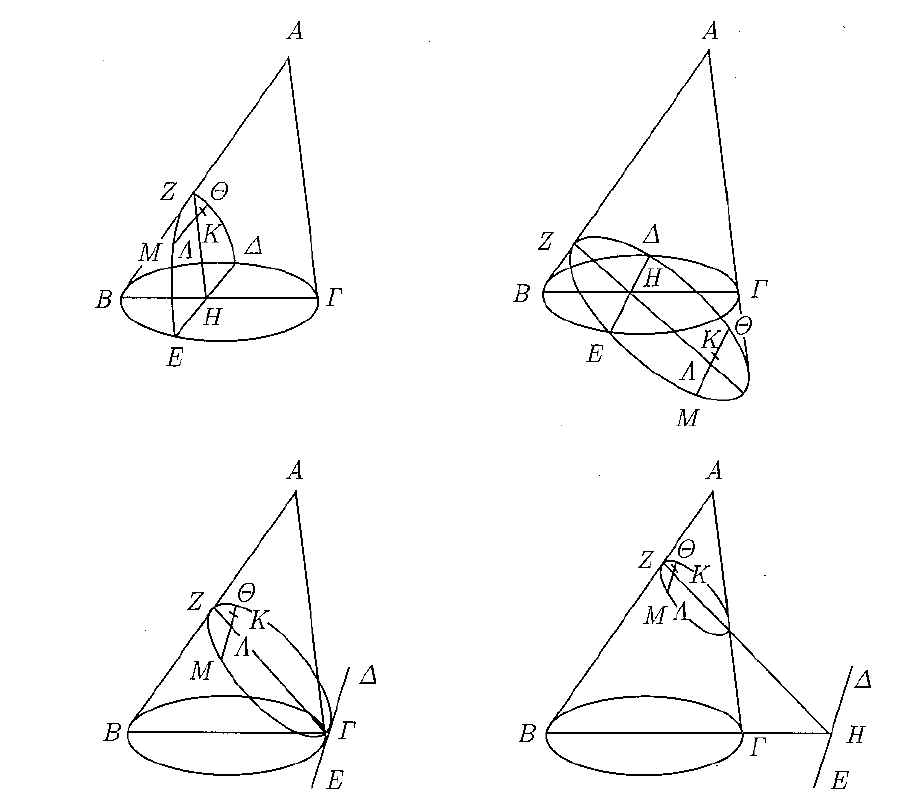
\includegraphics[width=\textwidth]{ConicsOfApollonius.png}

  \part{Operator Theory}
  \chapter{Operator Theory}

  \part{Geometry}
  \chapter{Geometry}

  \section{Introduzione}
Lo scopo di queste pagine è di mettere lo studente in grado di apprendere in maniera autonoma i concetti e gli strumenti della geometria.
Le pagine sono rivolte a studenti dei corsi di Matematica in quanto le conoscenze sono presentate sotto forma di definizioni, teoremi e relative dimostrazioni applicando le tecniche e gli strumenti della logica matematica.
I concetti, seppur presentati il più possibile in maniera formale, sono accompagnati da commenti scritti con il linguaggio dello studente.
Infatti, vengono associate al formalismo puro tipico della matematica moderna un linguaggio comune e comprensibile a tutti. Per questo si cerca di spiegare parola per
parola il significato dei termini delle definizioni, dei teoremi e di ogni altro enunciato. Le pagine di teoria sono accompagnate da
esercitazioni pratiche sia di esercizi ed esami svolti e sia di esercizi da svolgere in autonomia. Altro obiettivo è quello di contenere
in un'unica trattazione tutto il sapere matematico necessario per superare tutti gli esami di geometria proposti nei corsi universitari
di Matematica e di ogni altro corso di laurea che include anche lo studio della geometria. Le pagine sono strutturate in un indice in cui si trova
il syllabus (il nostro programma di studio) e di una pagina per ogni concetto. Le pagine sono scritte in latex e trasformate in html per la
visualizzazione. E' possibile convertire anche in formato pdf.

\subsection{I link}
Ogni pagina che espone un concetto contiene un certo numero di link. I link che mostrarno l'url, per esempio: \url{http://calvino.polito.it/~tedeschi/geometria/}, sono link 
esterni al documento. I link che non mostrano l'url, per esempio: \href{./GeometriaEuclidea.html}{Geometria euclidea}, sono link interni.
Se cliccate su un link esterno relativo a esercizi allora tutto bene ma se cliccate link esterni di teoria può darsi che la pagina non sia
completa o sia scritta in maniera non del tutto comprensibile. In quest'ultimo caso potete avvisare i partecipanti al progetto, aprendo un issue su github. 

\subsection{Prerequisites}
Costanza nello studio, dedicare il giusto tempo, meglio un pò al giorno tutti i giorni.




  \section{Geometria Euclidea}
La geometria Euclidea bla bla bla
%\section{Geometria Euclidea: definizione}
\begin{definizione}
Si chiama \emph{\bf{geometria euclidea}} la classica geometria che si studia alle scuole elementari, medie e superiori. E' quella che si basa sugli Elementi di Euclide dove
i concetti fondamentali (ovvero gli assiomi) sono quelli di punto, retta, etc.
\end{definizione}

\begin{definizione}
Si chiama \emph{\bf{segmento orientato (non banale)}} un segmento su cui sia stato scelto un verso, ovvero su cui si sia fissato un ordine tra i due estremi. 
\end{definizione}

\begin{definizione}
Si chiama \emph{\bf{segmento orientato banale}} \`e quello che inizia in un punto $A$ e finisce sempre in $A$.
\end{definizione}

\begin{definizione}
Si chiama \emph{\bf{insieme dei segmenti orientati}} l'insieme dei segmenti orientati.
\end{definizione}

\begin{osservazione}
Ovviamente l'insieme dei segmenti orientati \`contiene anche il segmento orientato banale per definizione.
\end{osservazione}

\begin{definizione}
L'\emph{\bf{equipollenza}} \`e una relazione di equivalenza tra due segmenti orientati dell'insieme dei segmenti orientati.
\end{definizione}

\begin{definizione}
Si chiama \emph{\bf{vettore geometrico dello (o nello) spazio}}
\end{definizione}

\section{Vettore}
\subsection{Vettore colonna, vettore riga}
Un vettore in uno spazio $n$-dimensionale è un insieme ordinato formato da $n$ valori. 

\subsection{Vettore in geometria mono, bi e tri-dimensionale}
Un vettore è un oggetto che ha una direzione e una lunghezza. In questo caso si dimostrerà che un vettore può essere
rappresentato come da definizione precedente.

\subsection{Componenti di un vettore}

\subsection{Rappresentazione canonica}

\subsection{Lunghezza di un vettore in $R^n$}
The length of a vector $v$ in $R^n$ is the square root of the sum of the squares of tis components.
\[
 |v|=\sqrt{v^2_1+...+v^2_n}
\]

This is a natural generalization of the Pythagorean Theorem.

\subsection{dot product or scalar product}
The dot product (or inner product or scalar product) of two $n$-component real vectors is the linear combination of their components.
\[
 u \dotfill v = u_1v_1+...+u_nv_n
\]
squares of its components.


\subsection{NOTAZIONE}

\subsection{NOTE}
Le due definizioni sono equivalenti nel senso che si possono rappresentare i vettori della definizione 2 come vettori
della definizione 1.

Attenzione alla definizione di vettore libero.

Attenzione all'uguaglianza tra due vettori. Due vettori sono uguali quando hanno la stessa rappresentazione canonica.




  \section{Algebra Lineare}



\section{Introduzione tratta dal libro "Introduzione all'algebra lineare" Prof. Fioresi-Morigi}
Le applicazioni lineari sono funzioni tra spazi vettoriali che ne rispettano la struttura, cioè sono compatibili con le operazioni di somma tra vettori e moltiplicazione di un
vettore per uno scalare. Come vedremo le applicazioni lineari si rappresentano in modo molto efficace attraverso le matrici. Lo scopo di questo capitolo è quello di introdurre
il concetto di applicazione lineare e capire come sia possibile associare univocamente una matrice ad ogni applicazione lineare tra $R^n$ e $R^m$, una volta fissata in entrambi
gli spazi la base canonica. Studieremo poi il nucleo e l'immagine di un'applicazione lineare fino ad arrivare al Teorema della dimensione, che rappresenta uno dei risultati più
importanti della teoria sugli spazi vettoriali di dimensione finita.




\subsection*{Syllabus Algebra Lineare}
\subsubsection{Spazi Vettoriali}
\begin{itemize}
 \item Vettore
 \item \href{CoordinateVettore.pdf}{Coordinate di un vettore}
 \item \href{SpazioVettoriale.pdf}{Spazio Vettoriale}
 \item Sottospazio vettoriale
 \item Combinazione lineare
 \item Spazio generato dai vettori $v_1, ..., v_k$
 \item Sistema di generatori
 \item Versore
 \item Interdipendenza lineare (Indipendenza lineare)
 \item \href{Base.pdf}{Base di uno spazio vettoriale}
 \item Base canonica
 \item Matrice di cambiamento di base
 \item Criterio di indipendenza
 \item Estrazione di una base
 \item Completamento a una base
 \item \href{Dimensione.pdf}{Dimensione di uno spazio vettoriale}
 \item Componenti
 \item Somma diretta e somma 
 \item Spazi quozienti
 \item Duale
\end{itemize}

\subsubsection{Matrici}
\begin{itemize}
   \item \href{Matrice.pdf}{Matrice}
   \item Matrici identit\'{a} (identica)
   \item Matrice nulla
   \item Matrice opposta 
   \item \href{InsiemeDelleMatrici.pdf}{Insieme delle matrici $m \times n$: $M_{m,n}(K)$}
   \item Matrice trasposta
   \item Properties of Transpose Matrices: \url{http://www.math.nyu.edu/~neylon/linalgfall04/project1/dj/proptranspose.htm}
   \item Help with proving that the transpose of the product of any number of matrices is equal to the product of their transposes in reverse.
   \item La trasposta della trasposta \'{e} la matrice stessa
   \item La trasposta della somma di due matrici è uguale alla somma delle due matrici trasposte
   \item L'ordine delle matrici si inverte per la moltiplicazione
   \item Se $c$ \'{e} uno scalare, la trasposta di uno scalare \'{e} lo scalare invariato
   \item Nel caso di matrici quadrate, il determinante della trasposta \'{e} uguale al determinante della matrice iniziale
   \item La trasposta di una matrice invertibile \'{e} ancora invertibile e la sua inversa \'{e} la trasposta dell'inversa della matrice iniziale
   \item Se $A$ \'{e} una matrice quadrata, allora i suoi autovalori sono uguali agli autovalori della sua trasposta
   \item \href{SommaMatrici.pdf}{Operazione di somma tra matrici}
   \item \href{ProdottoMatrici.pdf}{Operazione di prodotto tra matrici}
   \item Properties of matrix multiplication: \url{https://www.khanacademy.org/math/precalculus/precalc-matrices/properties-of-matrix-multiplication/a/properties-of-matrix-multiplication}
   \item Operazione di prodotto tra uno scalare ed una matrice
   \item \href{MatriceQuadrata.pdf}{Matrice Quadrata}
   \item \href{OrdineMatrice.pdf}{Ordine di una matrice quadrata}
   \item \href{DeterminanteMatrice.pdf}{Determinante di una matrice quadrata}
   \item \href{PolinomioMatrice.pdf}{Polinomio caratteristico di una matrice}
   \item \href{AutovaloriMatrice.pdf}{Autovalori di una matrice quadrata}
   \item \href{Autovalore.pdf}{Autovalore}
   \item Autovettore
   \item Molteplicità algebrica e geometrica
   \item Matrice diagonale
   \item \href{MatriceDiagonalizzabile.pdf}{Matrice diagonalizzabile}
\end{itemize}

\subsubsection{Sistemi lineari}
  \begin{itemize}
   \item Sistema di che cosa?
   \item Sistema lineare e matrici.
   \item Sistema lineare
   \item Sistema omogeneo
   \item Risoluzione
  \end{itemize}
  
\subsubsection{Applicazioni lineari}
  \begin{itemize}
   \item \href{IntroAppLineari.pdf}{Introduzione alle applicazioni lineari}
   \item Applicazione lineare
   \item Nucleo di un'applicazione lineare
   \item Immagine di un'applicazione lineare
   \item Base di un'applicazione linearea
   \item Cambio di base per un'applicazione lineare
   \item \href{ApplicazioneIniettiva.pdf}{Applicazione lineare iniettiva}
   \item \href{DimensioneImmagine.pdf}{Dimensione dell'immagine di un'applicazione lineare}
   \item Teorema della dimensione
   \item \href{MatriceApplicazione.pdf}{Matrice associata ad un'applicazione lineare tra spazi vettoriali}
   \item Isomorfismo di applicazioni lineari
   \item Calcolo del nucleo e dell'immagine
   \item Diagonalizzazione
   \item Applicazione lineare diagonalizzabile
  \end{itemize}


\section{DEFINIZIONE}
Un'applicazione lineare è iniettiva se il nucleo dell'applicazione è il vettore nullo.



\section{DEFINIZIONE}
La dimensione dell'imagine di un'applicazione lineare è uguale al rango 
della matrice associata all'applicazione lineare.



\section{DEFINIZIONE}
La matrice associata ad un'applicazione lineare tra spazi vettoriali si ottiene mettendo nelle colonne della matrice
le immagini dei vettori della base canonica del dominio (o di altra base data).

\section{NOTAZIONE}

\section{ESEMPIO}

\section{APPROFONDIMENTI}
\begin{itemize}
 \item \url{http://www.dm.unibo.it/~ida/NoteGeometria1-25-5-16.pdf}
 \item \url{http://joshua.smcvt.edu/linearalgebra/book.pdf}
 \item \url{http://www.youmath.it/lezioni/algebra-lineare/applicazioni-lineari/771-calcolare-dimensione-e-base-di-nucleo-e-immagine.html}
\end{itemize}


\section{Matrice}
$A = (a_{ij})_{i=1...m,j=1...n}$

la seguente notazione ritengo sia errata:
$A = a_{ij}$

Perch\'{e} stiamo cerchando di assegnare un elemento di una matrice ad una matrice.

Pertanto sarebbe corretto scrivere: $A = (a_{ij})$ oppure in maniera completa $A = (a_{ij})_{i=1...m,j=1...n}$


\section{DEFINIZIONE}
Matrice che ha lo stesso numero di righe e colonne.



\section{DEFINIZIONE}
L'ordine di una matrice quadrata è il numero di righe o equivalentemente il numero di colonne.

\section{ESEMPIO}
Una matrice quadrata con n righe ed e colonne ha ordine n.



\section{DEFINIZIONE}
Sia A una \href{./MatriceQuadrata.html}{matrice quadrata}, t una incognita (la nostra x) e $I_n$ la matrice identità di \href{./OrdineMatrice.html}{ordine} n. Il polinomio caratteristico (nella incognita $t$) di una matrice è uguale al \href{./DeterminanteMatrice.html}{determinante} della matrice:
\[
 A-tI_n
\]

scriviamo:
\[
 p_A(t) := det(A-tI_n)
\]



\section{Introduzione}
Sotto talune condizione riguardo ai tipi di matrice, cio\'{e} sul numero delle righe e delle colonne che le matrici che si intendono moltiplicare devono avere, definiamo un'operazione
che chiamiamo \textit{operazione di prodotto tra matrici} o \textit{prodotto tra matrici} o \textit{prodotto riga per colonna}.
Bene, diciamolo subito, tra tutte le matrici dell'insieme $M_{m,n}$ \'{e} possibile moltiplicare tra di loro quelle in cui il numero di colonne della prima matrice corrisponde al
numero di righe della seconda matrice. Per questo motivo viene chiamato prodotto righe per colonne.

Altra cosa da tenere presente \'{e} il fatto che la forma della matrice risultato pu\'{o} essere diversa da quella delle matrici che abbiamo moltiplicato. Ed infatti, la matrice risultato
sar\'{a} composta da $m$ righe ed $n$ colonne, dove, $m$ \`{e} il numero di righe della prima matrice e $n$ \`{e} il numero di colonne della seconda matrice.

\begin{definizione}
 Se $A$ \`{e} una matrice $m \times s$ e $B$ \`{e} una matrice $s \times n$, definiamo il prodotto $c_{ij}$ della riga $i$ di $A$ e della colonna $j$ di $B$ nel modo seguente:
 \[
  c_{ij} = \begin{pmatrix}
	      a_{i1} & ... & a_{is}
           \end{pmatrix}           
           \begin{pmatrix}
	      b_{1j} \\
	      ... \\
	      b_{sj}
           \end{pmatrix}
         = a_{i1}b_{1j} + ... + a_{is}b_{sj}
         = \sum_{h=1}^s a_{ih}b_{hj}
 \]

\end{definizione}

In altre parole, per ricavare l'elemento di posto $(i,j)$ bisogna eseguire il prodotto riga per colonna tra la riga $i$ e la colonna $j$.

Analogamente all'operazione di somma tra matrici, quello che \`{e} importante capire \`{e} quale formula \`{e} utilizzata per ricavare l'elemento di posto $(i,j)$. Solo che,
nel caso della somma tra matrici, l'operazione \`{e} banale ed immediata, qui invece l'operatore di sommatoria potrebbe dare qualche problema agli inizi, ma poi ci si fa l'abitudine.



\section{DEFINIZIONE}
L'operazione di somma tra matrici si effettua applicando l'operazione di somma del campo $K$ di cui sono fatti gli elementi delle matrici.
Le matrici devono avere lo stesso numero di righe e di colonne.

\section{SIMBOLI}
$A = B + C$

$a_{ij} = b_{ij} + c_{ij}$





\section{DEFINIZIONE}
Gli autovalori di una matrice quadrata sono le radici del polinomio caratteristico.




\section{DEFINIZIONE}
L'insieme delle matrici $mxn$: $M_{m,n}(K)$ ha una struttura di spazio vettoriale con l'operazione di somma tra matrici.


\section{Definizione (1)}
Una matrice quadrata $A$ si dice \textit{diagonalizzabile} se esiste una matrice invertibile $P$ tale che $P^{-1}AP$ sia diagonale.

\section{Definizione (2)}
Una matrice è diagonalizzabile se:
\begin{enumerate}
 \item Il numero degli autovalori, contati con la loro molteplicità, sia pari all'ordine della matrice.
 \item La molteplicità geometrica di ciascun autovettore coincida con la relativa molteplicità algebrica.
\end{enumerate}

\section{APPROFONDIMENTI}
\begin{itemize}
 \item \url{http://www.youmath.it/lezioni/algebra-lineare/matrici-e-vettori/1581-matrice-diagonalizzabile.html}
\end{itemize}



\section{DEFINIZIONE}
Si chiama Spazio Vettoriale una qualunque struttura matematica che possiede determinate propriet\'{a}.

\section{Descrizione}
Affinch\'{e} si possa parlare di spazio vettoriale occorrono almeno due insiemi generalmente indicati con $V$ e $K$. Tra gli elementi di $V$ \'{e} definita
una funzione che associa ad ogni coppia di elementi di $V$ un elemento di $V$. Tale funzione viene chiamata operazione di somma.
\section{Propriet\'{a}}


\section{ESEMPIO}
L'insieme dei numeri reali con l'operazione di somma con l'operazione di somma e prodotto.
L'insieme dei vettori geometrici dello spazio con l'operazione di somma tra vettori e prodotti di vettori per uno scalare.




\section{DEFINIZIONE}
A basis for a vector space is a sequence of vectors that is linearly independent and that spans the space.

\section{NOTE}
A vector space can have many different bases.

Tutte le basi hanno lo stesso numero di vettori.



\section{Definizione}
buona bibliografia qui: \url{https://it.wikipedia.org/wiki/Coordinate_di_un_vettore}




\section{DEFINIZIONE}
The dimension of a vector space is the number of vectors in any of its bases.



%  \section{Forme Bilineari}
\begin{itemize}
	\item Forme bilineari: Matrice associata a una forma bilineare. 
	\item Forme simmetriche e antisimmetriche. 
	\item Basi ortogonali. 
	\item Esistenza di basi ortogonali per le forme simmetriche. 
	\item Forme bilineari simmetriche reali. 
	\item Teorema di Sylvester. 
	\item Teorema spettrale reale. 
	\item Cenno alle forme hermitiane e al teorema spettrale complesso.  
	\item Coniche e quadriche di $R^n$ e loro classificazione affine ed euclidea.
\end{itemize}




  \part{Global analysis, analysis on manifolds}  
  \chapter{Global analysis, analysis on manifolds}


\chapter{Pareto Optimality}

\section{Pareto Optimality and Social Optimality. \cite{kleinberg2010}}

In a Nash equilibrium, each player's strategy is a best response to the other player's strategy....???

Pareto Optimality. The first definition is 

\section{Pareto Optimality. \cite{bauso2014}}
We conclude this chapter (chap.4) introducing a property which may or may not be enjoyed by equilibria, that is, Pareto optimality. 
It must be said that, equilibria that are also Pareto optimal represent extremely stable solutions in that not only no player is better off by changing actions, but also no players can be better off by jointly deviating without causing a loss for at least one player.

\quote{La cosa interessante is that pareto-optimality is defined as a property, e non importa se questa propriet\`a \`e in qualche modo connessa al concetto di equilibrio. Infine si ricorda che un equilibrio che sia anche pareto ottimale rappresenta l'eccezione e non la regola, semmai ci fosse una conessione di dipendenza tra il concetto di equilibrio e quello di paretto ottimalit\`a}

\begin{definizione}
	A pair of strategies $(a_{1}^{PO}, a_{2}^{PO})$ is said to be Pareto optimal (PO) if there exists no other pair $(a_1,a_2)$ such that for $i=1,2$
		\[
			u_i(a_1, a_2) > u_i(a_{1}^{PO}, a_{2}^{PO}) \wedge u_{-i} \ge u(a_{1}^{PO}, a_{2}^{PO}) 
		\]
\end{definizione}	

Ora che abbiamo la formula della pareto optimality non ci resta che applicarla ad un esempio concreto. 

\begin{verbatim}
	LET N be SET players
	Una volta stabilito il numero dei giocatori, tutte le tuple 
	hanno lunghezza |N|=:n
	n lo utilizziamo solo per il numero dei giocatori
	altri indici utilizzati saranno: i, j, d
	LET A be SET alternatives
	LET S be SET strategies WHERE s \in S = (a_1, ..., a_n) - 'a' for alternative(choice)
	LET P be SET prospects(outcomes) WHERE p \in P = (p_1, ..., p_n) - 'p' for payoff
	LET u be FUNCTION u : S --> P
	E.G. u(s) |--> (p_1, ..., p_n), p_1, ..., p_n \in R^n
	
	l'operatore su tuple t_{-i} restituisce una tupla di lunghezza di t meno 1.
\end{verbatim}

\begin{definizione}
	Una strategia si dice \emph{pareto-optimally} if there is no other strategy that adhere with the following conditions:
	\begin{enumerate}
		\item 
	\end{enumerate}
\end{definizione}




  
  \part{Probability}
  \chapter{Probability}

\chapter{Definition of Probability}

\section{Numero aleatorio}
bla

\section{Probabilities as set functions. \cite{rossi26102017}}
\begin{itemize}
 \item Conceptually, probabilities are associated with \emph{events or subsets} $A \in 2^X$ of atomic mutually exclusive events $x \in X$. 
       In fact, a probability distribution is a \emph{set function} satisfying $p(A)+p(B)=p(A \cap B) + p(A \cup B)$ for all $A,B \in 2^X$.
\end{itemize}

Quindi si richiede che gli elementi dell'insieme X dei possibili eventi (qui c\`e una certa ridondanza), piuttosto utilizzerei la terminilogia adottata da:

Intanto che cosa \`e un evento? Un evento \`e un numero aleatorio ossia un numero rappresentato da una lista non ordinata di valori.

Es. $x_1 = \{1,2,3,4,5\}$ oppure $x_2 = \{0,1\}$ oppure $x_3 = \{7\}$ $x_1$, $x_2$ e $x_3$ vengono chiamati numeri aleatori. $x_3$ pur essendo un insieme si potrebbe far corrispondere al numero $7$. $x_2$ si chiama evento perch\`e pu\`o assumere soltanto due valori $0$ e $1$.



  
  \part{Game theory, economics, social and behavioral sciences}
  \chapter{Game theory, economics, social and behavioral sciences}

\chapter{Computational Methods}

\begin{verbatim}
Vedi http://gambit.sourceforge.net/gambit15/gui.html
\end{verbatim}


\chapter{Game theory}

\section{ACHTUNG!}

Appunti personali presi durante il corso di Giochi e Modelli Booleani (aka Teoria dei giochi (TG)) - 82114 - ANNO 2017/18 - tenuto dal Prof. Giovanni Rossi. Non avendo seguito tutto il corso, alcuni fatti potrebbero risultare distorti mentre altri potrebbero tornare utili.

\section{Todos}
In questa sezione ci sono le cose ancora da sistemare.
vedi \cite{vorobev01} pag.2 for constant sum game

Vedi capitolo 6 per descrizione gioco e primo approccio alla probability

%% SETS

%% SETS IN GENERAL


%% SETS FOR GAMES MODELING
\newcommand{\actionSet}{A_i = \{ a_{i}^{1, ..., a_{i}^{|A_i|}} \}}
\newcommand{\actionProfileSet}{A = A_1 \times ... \times A_n}
\newcommand{\alternativeSet}{ X = \{x_1, ..., x_m\}}
\newcommand{\playerSet}{ N = \{1, ..., n\} }
%\newcommand{\100playerSet}{ N = \{1, ..., 100\} }
\newcommand{\powerSet}{2^N}
\newcommand{\eventSet}{2^X}
\newcommand{\realSet}{\mathbb{R}}
\newcommand{\nonnegativeRealSet}{\mathbb{R}_{+}}   %% [0,infty) quindi zero compreso
\newcommand{\positiveRealSet}{\mathbb{R}_{++}}     %% (0,infty) quindi escluso lo zero
\newcommand{\strategySet}{S_i = \{ 0, 1 \}}
\newcommand{\strategySets}{S_1 = \{s_{i}^{1}, ..., s_{i}^{|S_i|}\}}

%% SETS FOR GRAPH MODELS
\newcommand{\edgeSet}{\mathbb{E}}
\newcommand{\vertexSet}{\mathbb{V}}
\newcommand{\vertexList}{\{v_0, v_1, ..., v_{|\vertexSet|-1}\}}


%% FUNCTIONS
\newcommand{\setFunction}{p:2^X \to [0,1]}
\newcommand{\utilityFunction}{u_i:\strategies \to R}

%% TUPLE SET - ORDERED LIST
\newcommand{\strategies}{S_1 \times ... \times S_n}

%% OBJECTS / POINTS / ELEMENTS
\newcommand{\strategy}{s = (s_1, ..., s_n)}

%% SET AS UNORDERED LIST
\newcommand{\events}{X}

%% GAMES
\newcommand{\coopCoalGame}{v: \powerSet \to \realSet}         %% is a cooperative coalitional game
\newcommand{\gameTree}{\mathfrak{T} = (\vertexSet, \edgeSet)} %% is a multistage game
%%, V=\{v_0,v_1,...,v_{|V|-1}\}, E \subseteq V \times V }

\chapter{Preface}
\chapter{How to study Game Theory}
La teoria dei giochi deve essere studiata da due angolazioni, da due facce della stessa medaglia potremmo dire forzando un p\`o la fantasia. Ossia, il punto di vista della realt\`a che si vuole modellare, quindi per esempio l'economia ed il punto di vista del modello matematico sottostante. \`E chiaro che i due punti di vista hanno approcci e metodi differenti ma non \`e solo questo il punto. La dicotomia si concretizza nel fatto che l'insieme dei player sia rappresentato, per esempio, dal player set: $\playerSet$. Cio\`e una volta stabilita la corrispondenza uno a uno, biunivoca tra realt\`a e matematica, possiamo tralasciare il punto di vista della real\`a ovvero possiamo disinteressarcene e prendiamo a considerare soltanto l'oggetto matematico rappresentato in questo caso dal player set $\playerSet$. Se considero l'insieme power set $\powerSet$, che cosa sto facendo? Dal punto di vista della matematica una cosa assolutamente lecita, devo capire di cosa si tratta e come faccio a manipolarla e dal punto di vista del ritorno alla realt\`a posso dire in questo caso che $\powerSet$ rappresenta l'insieme di tutte le possibili coalizioni di giocatori. Il power set lo vedremo e rivedremo quindi niente paura.

Ed infatti i padri della disciplina parlano di shift (spostamento) da teoria economica a matematica (e viceversa), cio\`e lo spostamento da realt\`a a modello matematico.

\section{Shift of Emphasis from Economics to Games. \cite{vonNeumann1944}}
Chapter II, GENERAL FORMAL DESCRIPTION OF GAMES OF STRATEGY, 5. Introduzione, 5.1 Shift of Emphasis from Economics to Games, \cite{vonNeumann1944}.

\quote{It should be clear from the discussions of Chapter I that a theory of rational behaviour - i.e. of the foundations of economics and of the main mechanisms of social organization - requires a thorough study of the "games of strategy." Consequently we must now take up the theory of games as an independent subject. In studying it as a problem in its own right, our point of view must of necessaty undergo a serious shift. In Chapter I our primary interest lay in economics. It was after having concived ourselves of the impossibility of making progress in that field without a previous fundamental understangin of the games that we gradually approached the formulations and the questions which are partial to that subject. But economic viewpoints remained nevertheless the dominant ones in all of Chapter I. From this Chapter II on , however, we shall have to treat the games as games. Therefore we shall not mind if some points taken up have no economic connections whatever, - it would not be possible to do full justice to the subject otherwise. Of course most of the main concepts are still those familiar from the discussions of economic literature (cf. the next section) but the deails will often be altogether alien to it - and details, as usual, may dominate the exposition and overshadow the guiding principles.}

\chapter{Introduction to Game Theory}
\begin{itemize}
	\item Game theory "begins" in 1944 with the book $[32]$ Games and Economic Behavior by von-Neumann and Morgestern.
	
	\item In 1953 Shapley publishes a fundamental paper $[27]$ defining cooperative games, so that the former ones have been named "non-cooperative" (or strategic) ones thereafter.
	
	\item Given a set $N=\{1,...,n\}$ of $n$ players, a non-cooperative game consists of a product space $S_1 \times ... \times S_n$ of strategies, and $n$ utilities or payoff functions $u_i:S_1 \times ... \times S_n \to R$, $1 \le i \le n$ measuring the "goodness" of strategy profiles $s \in S_1 \times ... \times S_n$ to players $i \in N$. This is the branch of game theory where the famous prisoner's dilemma and Nash equilibrium apply. On the other hand, a cooperative (coalitional) game is a set function $v:2^N \to R_+$ such that $v(0)=0$, where $2^N = \{A:A \subseteq N\}$ is the $2^n$-set of coalitions $A$ or subsets of $N$. Specifically, $v(A)$ is thought of as the worth of cooperation among all (and only) players $i \in A$ (or coalition members).
	\begin{enumerate}
		\item Perch\`e 2?
		\item Ha senso la coalizione in cui sono presenti tutti i players?
	\end{enumerate}
	\item ...
\end{itemize}
\chapter{Games classification}
Come sono classificati i giochi? Cio\`e qual'\`e la terminologia adottata se facciamo variare alcune variabili/propriet\`a dei termini/oggetti coinvolti ossia players, randomizzazione, payoffs, alternative.

\section{General Principles of Classification and of Procedure. \cite{vonNeumann1944}}
Chapter II, GENERAL FORMAL DESCRIPTION OF GAMES OF STRATEGY, 5 Introduction, 5.2 General Principles of Classification and of Procedure.

[5.2.1.] Certain aspects of "games of strategy" which were already prominent in the last sections of Chapter I will not appear in the beginning stages of the discussions which we are now undertaking. Specifically: There will be at first no mention of coalitions between players and the compensations which they pay to each other. (Concerning these, cf. 4.3.2., 4.3.3., in Chapter I).

Per cui all'inizio trascuriamo il fatto che i giocatori possano cmq aiutarsi gli uni e gli altri. Da qui la principale suddivisione ossia tra giochi cooperativi e giochi non cooperativi. In realt\`a nel testo \cite{vonNeumann1944} la prima distinzione fondamentale \`e tra giochi a somma zero (mors tua vita mea) e giochi a somma diversa da zero, diciamo positiva. Ma cosa devo sommare?. Nel testo "The computational beauty of nature" si parla di competizione e cooperazione.

We give a brief account of the reasons, which will also throw some light on our general disposition of the subject.

An important viewpoint in classifying games is this: Is the sum of all payments received by all players (at the end of the game) always zero; or is this not the case? If it is zero, then one can say that the players pay only to each other, and that no production or destruction of goods is involved. All games which are actually played for enternainment are of this type. But the economically significant schemes are most essentially not such. There the sum of all payments, the total social product, will in general not be zero, and not even constant. I.e., it will depend on the behavior of the players - the participants in the social economy. This distinction was already mentioned in 4.2.1., particularly in footnote 2, p.34. We shall call games of the first-mentioned type \emph{zero-sum} games, and those of the latter type \emph{non-zero-sum} games.

We shall primarily construct a theory of the zero-sum games, but it will be found possible to dispose, with its help, of all games, without restriction. Precisely: We shall show that the general (hence in particular the variable sum) $n$-person game can be reduced to a zero-sum $n+1$-person game. (Cf. 56.2.2.) 

Wow calma un attimo. Di cosa stiamo parlando? Induzione matematica? cio\`e da dove saltano fuori $n$ ed $n+1$?

Now the theory of the zero-sum $n$-person game will be based on the special case of the zero-sum two-person game. (Cf. 25.2). Hence our discussion will begin with a theory of these games, which will indeed be carried out in Chapter III.

Now in zero-sum two person games coalitions and compensantions can play no role. 

The only fully satisfactory "proof" of this assertion lies in the construction of a complete theory of all zero-sum two-person games, whithout use of those devices. This will be done in Chapter III, the decisive result being contained in 17. It ought to be clear by common sense, howerver, that "understandings" and "coalitions" can have no role here: Any such arrangement must involve at least two players - hence in this case all players - for whom the sum of payments is identically zero. I.e. there are no opponents left and no possible objectives.

The questions which are essential in these games are of a different nature. These are the main problems: How does each player plan his course - i.e. how does one formulate an exact concept of a strategy? What information is available to each player at every stage of the game? What is the role of a player being informed about the other player's strategy? About the entire theory of the game?
\chapter{What is a game?}
In questa sezione proviamo ad descrivere il gioco... 
Arriviamo addirittura a concludere che non \`e necessario alcuna "classificazione" among games because there exists just one true story about definition of game and was given by \cite{vonNeumann1944}.

\section{The Elements of the Game. \cite{vonNeumann1944}}
Chapter II, GENERAL FORMAL DESCRIPTION OF GAMES OF STRATEGY, 6 The Simplified Concept of a Game, 6.2. The Elements of the Game

Let us now consider a game $\Gamma$ of $n$ players who, for the sake of brevity, will be denoted by 1, ..., n. The conventional picture provides that this game is a sequence of moves, and we assume that both the number and the arrangement of these moves is given \emph{ab initio}.We shall see later that these restrictions are not really significant, and that they can be removed without difficulty. For the present let us denote the (fixed) number of moves in $\Gamma$ by $v$ - this is an integer $v=1,2,...$. The moves themeselves we denote by ... capire che cavolo \`e quella Mmm???TODO

\section{Rappresentazione matematica degli elementi di un gioco}
\begin{itemize}
 \item Player/s          = SET
 \item Prospetto/outcome = ENNUPLA. e.g. $(x)$, $(a,b)$ dove $a, b, x$ sono variabili logiche, al posto delle quali pu\`o andare un nostro tipo matematico a scelta.
 \item Strategia         = ENNUPLA
 \item Utility Function  = Data una strategia, restituisce un prospetto.
 \item Ordine            = Serve per discernere le mosse dell'avversario e per ordinare le mie preferenze.
 \item Game              = $\setFunction$ - dato un insieme di players restituisce true se l'insieme soddisfa le regole del gioco.
 \item Rules             = sono le specifiche implementazioni che diamo alla utiliti function e a tutto il resto.
\end{itemize}


Dovevo aspettermelo che con von Neumann saltava fuori qualche sorta di assiomatizzazione. Ed infatti...
\chapter{Axiomatic Formulation (of a Game).}
\chapter{Preferences}
\section{Preferences}
\begin{itemize}
	\item In non-cooperative games (see above), the product space $\strategies = X$ of strategies, over which every player $i \in N$ has preferences in the form of a utility function $\utilityFunction$, is finite (unless otherwise specified).
\end{itemize}

\subsection{Rational preferences}
\begin{itemize}
	\item The primitive ingredient of a choice problem is a set $X$ of alternatives, which may be finite or infinite, and in this latter case either countable or uncountable.
			\begin{enumerate}
				\item L'insieme $X$ di questo punto e the product space $\strategies = X$ sono due cose completamente diverse, giusto?
				\item Qui $X$ \`e un generico insieme e quindi potrebbe anche essere quello del punto precedente? L'importante, come vedremo, che sia definita una relazione di preferenza?
			\end{enumerate}
		
	\item When denoting a finite alternative set by $X = \alternativeSet$, the first $m$ natural numbers $1, ..., m \in N$ are used as distinct "names" for the $|X|=m$ distinct alternatives.
\end{itemize}

\subsection{Utility representation}
\chapter{Randomness}
\begin{itemize}
 \item The next step in the study of non-cooperative games is the understanding of strategies. As we shall see, the famous Nash equilibrium surely exists only when players $i \in N$ may each randomize over their finite strategy sets $\strategySets$.
\end{itemize}

\section{Discrete random variables: lotteries}
\begin{itemize}
 \item ...
 \item By the way, also recall that a probability distribution over $X$ is defined as any set function $\setFunction$ satisfying $p(A)+p(B)=p(A \cap B)+p(A \cup B)$ for any two events or subsets (of elementary mutually exclusive events) $A, B \in 2^X$, as well as $p(X)=1$, $p(\o)=0$; then, a main theorem on valuations of distributive lattices (such as Boolean lattice $2^X, \cap, \cup)$) $[1, p. 190]$ entails $p(A) = \sum_{i \in A}p(\{i\})$ for all $A \in 2^X$ (this will be detailed when dealing with the \emph{solution} of coalition (cooperative) games $v:2^N \to R$, see below).
     \begin{enumerate}
      \item Che significa $p(A)+p(B)=p(A \cap B)+p(A \cup B)$?
      \item $[1, p. 190]$ cosa dovrei trovare? non ho capito?
     \end{enumerate}

\section{Probabilities, set functions and voting games}
	\begin{itemize}
		\item Recall that the quantitative notion of probability is associated with \emph{events or subsets $A \in 2^X$ of elementary, mutually exclusive (atomic) events.} In 
	\end{itemize}

\end{itemize}
\chapter{Strategies v. 10/10/2017}
\begin{itemize}
	\item In simultaneous-move games all player move or take action simultaneously, hence choosing a strategy is the same as choosing an action. This is no longer true in multistage games, where choosing a strategy means choosing a sequence of (conditional) actions. Although in this course non-cooperative games shall be dealt with only in simultaneous-move form, still multistage games are briefly introduced hereafter to formalize both a general definition of strategies and the notion of (in)complete information.
	\item I - baudo - Multistage games vengono introdotti per generalit\`a e per modellare la nozione di (in)complete information.
	\item before describing multistage games, the simultaneous-move setting enables to distinguish beetween outcomes of the game and strategy/action profiles. To this end, let each player $i \in N$ choose an action from a finite set $\actionSet$, where $|A_i| \ge 2$ for all $i \in N$. The product space $\actionProfileSet$ contains all $n$-tuples or profiles of actions, with generic element $a = (a_1, ..., a_n) \in A$. Preferences  
\end{itemize}


\subsection{Multistage games}
\subsection{Dominated and dominant strategies}
\subsubsection{Strategy deletion}
\subsubsection{Prisoner's dilemma}

\section{Randomization and expected payoffs}
\subsection{Mixed strategies}
\subsection{Domination in mixed strategies}
\subsection{Best responses}
\subsection{Nash equilibrium}
\subsection{Strong equilibrium}
\chapter{Strategies v. 26/10/2017}
Il concetto di strategia varia a seconda del tipo di gioco. Cosa vuol dire che il concetto varia? Vuol dire che a seconda del gioco \`e rappresentato da un certo tipo di oggetto matematico. 
Quasi sempre comunque la strategia \`e un elemento di un insieme pi\`u o meno complesso. Quindi secondo questo ragionamento l'alternative set, strategy set, action profiles, etc. sono tutte strutture matematiche che possono essere annoverate tra quelle che rappresentano il concetto di strategia del mondo reale ed i cui elementi sono, appunto, strategie. \\

Cominciamo con gli appunti del Prof. Giovanni Rossi (\cite{rossi26102017}).

\begin{itemize}
	\item In \emph{simultaneous-move games} alla players move only once, simultaneously, hence choosing a strategy is the same as choosing a move. This is no longer true in \emph{multistage games}, where choosing a strategy means choosing a \emph{sequence of (conditional) moves}. Although the non-cooperative games to be dealt with shall be in simultaneous-move form, still multistage games are briefly described below in order to formally define strategies in a most general setting, namely where players have either perfect or else incomplete information, this latter being commonly modeled by means of partitions.
\end{itemize}

\section{Information in multistage games}

\begin{itemize}
	\item As the name clearly suggests, multistage games are played in discrete time $t = 0, 1, ..., T$, as $t = 0$ is the starting point or \emph{root of the game tree} (defined hereafter), where some (at last one, and possibly all) players move; next, depending on previous moves, at each $t \ge 1$ a \emph{node} is reached, corresponding either to a moment where at least one player has to move, or else to an end of the game or \emph{leaf}. The concern is only with games where $T < \infty$ (for any leaf).
	
	\item Multistage games are thus commonly represented by a \emph{rooted and directed (game) tree} $\gameTree$, $\vertexSet = \vertexList$
\end{itemize}




\section{Dominated and dominant strategies}
\section{Deletion of dominated strategies}
\section{Equilibrium}
\chapter{Strategy}
Che cos'\`e una strategia? Valuta i prospetti. Tutti i prospetti. Supponi per un attimo di essere un essere superiore e di conoscere tutti i possibili risultati dell'interazione tra due entit\`a. Ops, scusate stavo correndo troppo. Supponiamo che le entit\`a siano invece due persone, la persona (o player) $p_1$ e la persona $p_2$.
Bene che cosa puoi fare? Bh\`e puoi pensare per esempio questo: "Se solo i giocatori conoscessero tutti i possibili esiti del gioco, di sicuro farebbero la scelta/mossa/strategia giusta". Ed infatti, per certi aspetti, nella teoria dei giochi \`e proprio cos\`i. Si dice con linguaggio tecnico che i players conoscono tutti i possibili prospetti(da prospetto: guardare innazi) del gioco. Se i giocatori hanno la possibilit\`a di guardare tutti i prospetti (anche se randomizzati) allora si dice che il gioco \`e ad \emph{informazione perfetta}, altrimenti, se alcuni prospetti non sono noti per qualche giocatore, allora il gioco si dice ad \emph{informazione incompleta}.  

Prima di addentrarci in formalismi che riguardano insiemi, ennuple, sottoinsiemi e mappe, lasciamo la parola a chi ha iniziato la discipline della teoria dei giochi.

\section{Explanation of the Termini Technici. \cite{vonNeumann1944}}
Chapter II, GENERAL FORMAL DESCRIPTION OF GAMES OF STRATEGY, 6 The Simplified Concept of a Game, 6.1 Explanation of the Termini Technici.

Before an exact definition of the combinatorial concept of a game can be given, we must first clarify the use of some termini. There are some notions which are quite fundamental for the discussion of games, but the use of which in everyday language is highly ambiguous. The words which describe them are used sometimes in one sense, sometimes in another, and occasionally - worst of all - as if they were synonyms. We must therefore introduce a definite usage of \emph{termini technici}, and rigidly adhere to it in all that follows.

First, one must distinguish between the abstract concept of a \emph{game}, and the individual \emph{plays} of that game. The \emph{game} is simply the totality of the rules which describe it.

\begin{definizione}
 A \emph{game} is the totality of the rules which describe it.
\end{definizione}

Every particular instance at which the game is played - in a particular way - from beginning to end, is a \emph{play}. In most games everday usage calls a play equally a game; thus in chess, in poker, in many sports, etc. In Bridge a play corresponds to a "rubber" in Tennis to a "set" but unluckily in these games certain components of the play are again called "games". The French terminology is tolerably unambiguous: "game" = "jeu", "play" = "partie".

Second, the corresponding distinction should be made for the moves, which are the component elements of the game. A move is the occasion of a choice between various alternatives, to be made either by one of the players, or by some device subject to chance, under conditions precisely prescribed by the rules of the game. The \emph{move} is nothing but this abstract "occasion", with the attendant details of description, - i.e. a component of the "game". The specific alternative chosen in a concrete instance - i.e. in a concete \emph{play} - is the \emph{choice}. Thus the moves are related to the choices in the same way as the game is to the play. The game consists of a sequence of moves, and the play of a sequence of choices. In this sense we would talk in chess of the first move, and of the choice "E2-E4".

Finally, the \emph{rules} of the game should not be confused with the \emph{strategies} of the players. Exact definitions will be given subsequently, but the distinction which we stress must be clear from the start. Each player selects his strategy - i.e. the general principles governing his choices - freely. 
While any particular strategy may be good or bad - provided that these concepts can be interpreted in an exact sense (cf. 14.5. and 17.8-17.10.) - it is within the player's discretion to use or to reject it. The rules of the game, however, are absolute commands. If the are ever infringed, then whole transaction by definition ceases to be game described by those rules. In many cases it is even physically impossible to violate them. E.g.: In Chess the rules of the game forbid a player to move his king into a position of "check". This is a prohibition in the same absolute sense in which he may not move a pawn sideways. But to move the king into a position where the opponent can "checkmate" him at the next move is merely unwise, but not forbidden.

\section{Rappresentazione matematica della strategia}
Generalmente una strategia (strategy profile) \`e una ennupla formata dalle strategie (strategy/alternative) dei singoli giocatori.

\section{Dominant and dominated strategies}
Let $x = (x_1, ..., x_n)$ and $y = (y_1, ..., y_n)$ be two different strategies, then $x$ pareto domina $y$ iif $x_i \le y_i$ for all $i \in N$. 
\chapter{Zero-Sum Games}

\section{Preliminary Survay. \cite{vonNeumann1944}}

\subsection{General viewpoints. \cite{vonNeumann1944}}

\subsection{The one-person game. \cite{vonNeumann1944}}

\subsection{Chance and probability. \cite{vonNeumann1944}}

\subsection{The next objective. \cite{vonNeumann1944}}
\chapter{Non-Zero-Sum Games}
\chapter{Esercitazione 1}
Nell'esercizio vedremo alcuni concetti visti durante la prima parte del corso del Prof. Giovanni Rossi.

%\begin{abstract}
%Appunti personali presi durante il corso di Giochi e Modelli Booleani (aka Teoria dei giochi (TG)) - 82114 - ANNO 2017/18 - tenuto dal Prof. Giovanni Rossi. Non avendo seguito tutto il corso, alcuni fatti potrebbero risultare distorti mentre altri potrebbero
%presentare delle lacune.  
%\end{abstract}

%%\input{chapters/preface.tex}
\chapter{Definitions}
Cominiciamo col dare le definizioni dei concetti che vengono impiegati nell'esercizio. \\
Per \emph{definizione} intendiamo una formula vera nel linguaggio della matematica basata sugli assiomi della teoria degli insiemi. \\

\section{Pareto}
Pareto cosa? Allora non avendo ben chiaro in mente di cosa andremo a parlare, tuttavia il processo di apprendimento per il tramite della funzione di ripartizione naturale aggrega,
sotto il sostantivo oggettivato \emph{pareto}, alcuni fatti.

Vediamo i fatti separatamente. Utilizzeremo da qui in avanti la p minuscola per indicare che l'entit\`a reale del modello o l'oggetto matematico sottostante possiedono le propriet\`a 
richieste per essere considerate \emph{pareto}.

\subsection{pareto-dominates}


\chapter{Types of cooperative games}


	Although in the 70s attention has also been placed on cooperative games with a continuum of players in terms of measure theory (see [5] and related literature), nowadays cooperative games are for the most part dealt with in terms of a finite player set, usually denoted by $N = \{1,...,n\}$. In particular, these games are approached through discrete mathematics as poset/lattice functions. That is, as real-valued functions defined on finite ordered structures. 
	
	%\begin{itemize}
		%\item Continuum of players vuol dire insieme infinito di giocatori oppure insieme finito/infinito di giocatori che pu\`o crescere fino all'infinito? 
		%\item Nel caso moderno, cio\`e attraverso l'utilizzo di insiemi finiti e ordinati, nei ragionamenti l'insieme iniziale dei giocatori rimane fisso oppure può crescere?
		%\item Measure theory? A measure is a generalization of the concepts of length, area, and volume. 
		%\item In [5] what's "value concept"?
		%\item Edgeworthian? 
		%\item Per il momento questo mi basta!!! Il punto introduce quello che servir\`a sapere in seguito: ordered set/lattices e funzioni definite a partire da questi insiemi all'insieme dei numeri reali. Per ulteriori approfondimenti sui giochi with a continuum of players vedi [5] e letteratura affine.
		%\item Since about 1960, attention has focused more and more on games with large masses of players, in which no individual player can affect the overall outcome. Such games arise naturally in the social sciences, as models for situations in which there are large numbers of very "small" individuals, like consumers in an economy or voters in an election. Mathematically, it is often convenient to represent these games with the aid of a "continuum" of players - like the continuum of points on a line or the continuum of drops in a liquid. Represented thus, such games are called non-atomic.[5]
		%\item Quindi i nostri giochi sono atomici?
	%\end{itemize}
		
	Historically, the first cooperative games were defined in 1953 [27] as set functions $v : 2^N \to R_+,v(0)=0$, with subsets $A \in 2^N$ referred to as coalitions (of players). These games may thus be called coalition games, although in many articles and books they are simply named cooperative games, as if exhausting the whole class of cooperative games.
			\begin{enumerate}
				\item Coalition games sono un tipo di cooperative game?
				\item $2^N$ ? qual \`e il significato di questa notazione?
				\item Prospetto?
				\item Essential games?
			\end{enumerate}
	
	Subsequently, in 1963, a further type of cooperative games entered the picture, involving partitions of players or coalition structures, i.e. partitions $P = \{A_1, ..., A_{|P|}\}$ of $N$. In particular, these second-generation cooperative games were named games in partition function form, and they are real-valued functions defined on pairs $(A, P)$ such that $A \in 2^N$ and $P$ is a partition of $N$ such that $A \in P$. These pairs $(A,P)$ are now referred to as "embedded coalitions" (or "embedded subsets" $[13, 14]$). These games pose serious problems in terms of lattice theory, as the corresponding ordered structure (i.e. of embedded subsets) currently needs ad hoc techniques for yielding a lattice (which in any case is not a geometric one, see below). 
			\begin{enumerate}
				\item ...
			\end{enumerate}
		
	Finally, in 1990, a third type of cooperative games was introduced and named "global games" $[12]$. These are simply real-valued partition functions, but still lead to embarassing results when it comes to define and quantify the so-called "solution". Roughly speaking, a solution of a cooperative games should determine the a priori worth, for each player, of playing the game. Somehow overcoming the mainstream literature, in the sequel we shall interpret solutions of cooperative games (of any kind) in terms M\''{o}bius inversion and atomic/geometric lattices.
			\begin{enumerate}
				\item "of any kind" si rifesce ai tre tipi di giochi cooperativi o a tutti i giochi, sia cooperativi che non cooperativi?
			\end{enumerate}	

\chapter{Order: posets and lattices}
\section{Order: posets and lattices}



	
	Our concern is only with posets or ordered structures which are:
	  \begin{enumerate}
	    \item finite, i.e. $|X|<\infty$,
	    \item with a bottom element $x_{\bot} \in X, i.e. x \ge x_{\bot}$ for all $x \in X$,
	    \item with a top element $x^{\top} \in X$, i.e. $x^{\top} \ge x$ for all $x \in X$.
	  \end{enumerate}
	  In particular, in the sequel our main concern shall be with the poset $(X, \ge)$ given by $(2^N, \supseteq)$ for a finite (player set) $N = \{1,...,n\}$.
	    \begin{enumerate}
	     \item Quindi il top del poset $(2^N, \supseteq)$ is equals to $2^N$ and the bottom of $(2^N, \supseteq)$ is equals to $\O$. 
	    \end{enumerate}
	    
	
	
	For all $x, y \in X$, the corresponding \emph{\bfseries{interval}} (or \emph{\bfseries{segment}} $[25]$) is the subset $[x,y]=\{z:x \le z \le y\} \subseteq X$; hence $x \le y \Rightarrow [x,y] \ne \O$ while $[y,x] = \O$.
	
	D - (baudo) - A partially ordered set is \emph{\bf{locally finite}} if each of its intervals has only finitely many elements.
	
	A chain is a subset $K \subset X$ any two of whose elements are comparable, i.e. for all $x, y \in K$, either $[x,y] \ne \O$ or else $[y,x] \ne \O$ hold.
	
	Dually, an antichain is a subset $AK \subset X$ any two of its elements are uncomparable, i.e. for all $x,y \in AK$, both $[x,y]=\O$ and $[y,x]=\O$ hold.
	
	The length of a chain $K = \{x_0,...,x_k\}$ is $|K|-1=k$.

	The covering relation, denoted by $>*$, is defined as follows: \\
	      $x>*y \Leftrightarrow [y,x]=\{x,y\}$ (where $\{x,y\} = \{y,x\}$) for all $x,y \in X$.
		  \begin{enumerate}
		   \item Vorrei capire la direzione/terminologia. Anche rispetto al libro!?
		   \item Todo - copiare appunti dal quaderno
		  \end{enumerate}
	
	For $z \ge y$, a $(z-y)$-chain $K_{*}^{z-y} = \{y=x_0, x_1, ..., x_k = z\}$ is said to be maximal if $x_l >* x_{l-1}$ for all $0 < l \le k$.
	    \begin{enumerate}
	     \item from the free dictionary: A sequence of $n+1$ subsets of a set of $n$ elements, such that the first member of the sequence is the empty set and each member of the sequence is a proper subset of the next one.
	    \end{enumerate}

	    
	If for any $y, z \in X$ all maximal $(z-y)$-chains have the same length, then poset $(X, \ge)$ is said to satisfy the Jordan-Dedekind JD condition, in which case for every element $x \in X$ the length of any maximal $(x-x_{\bot})$-chain is the \emph{rank} of $x$. Formally, for any poset $(X, \ge)$ with bottom element $x_{\bot}$ and satisfying the JD condition, the rank function $r: X \to Z_+$ is defined recursively by
	
	\begin{enumerate}
	 \item $r(x_{\bot}) = 0$
	 \item $x >* y \Rightarrow r(x) = r(y)+1$.
	\end{enumerate}
	Thus the rank measures the height of elements (in the Hasse diagram, see above and below).




APPUNTI UTILI PER QUESTA SEZIONE
\begin{itemize}
  \item Let $P$ be an ordered set. We say $P$ has a \emph{\bf{top}} element if there exists $\top \in P$ with the property that $x \le \top$ for all $x \in P$.
  \item uniquiness of the top (think of duality), antisymmetry etc.? Il top dovrebbe essere unico perch\`e se supponiamo che esista un altro top $t2$ tale che quindi $x \le t2$ for all $x \in P$ ma allora si avrebbe $\top \le t2 \Rightarrow t2 !\le \top$ per la propriet\`a antisimmetrica pertanto siamo giunti ad una contraddizione perch\`e avevamo supposto $\top$ essere un top. 
  \item Let $P$ be an ordered set and let $S \subseteq P$. An element $x \in P$ is an \emph{\bf{upper bound}} of $S$ if $s \le x$ for all $s \in S$.
  \item Upper bound is unique when it exists.
  \item Quindi posso dire che un top \`e un upper bound che sta dentro l'insieme $P$? Insomma che differenza c\`e tra upper bound e top?
  
  \item In a partially ordered set, an element $p$ emph{covers} an element $q$ when the segment $[q,p]$ contains two elements. $[25, 343]$
  
  \item A lattice is a partially ordered set where max and min of two elements (we call them join and meet, as usual, and write $\vee$ and $\wedge$) are defined. $[25, 342]$
  
  \item A \emph{\bf{segment}} $[x,y]$, for $x$ and $y$ in a partially ordered set $P$, is the set of all elements $z$ between $x$ and $y$, that is, such that $x \le z \le y$. ... . A segment is endowed with the induced order structure; thus, a segment of a lattice is again a lattice. $[25, 342]$
  
  \item A partially ordered set is \emph{\bf{locally finite}} if every segment is finite. $[25, 342]$
  
  \item Let $P$ be a non-empty ordered set. \\
        If $x \vee y$ and $x \wedge y$ exist fora all $x, y \in P$, then $P$ is called a \emph{\bf{lattice}}. \\
        If $\vee S$ and $\wedge S$ exist for all $S \subseteq P$, then $P$ is called a \emph{\bf{complete lattice}}.
        
  \item Totally ordered subsets of a poset play an important role in the theory of partial orders.
  
  \item 
\end{itemize}

\subsection{Maximal chains of subsets and permutations}
\subsection{Subset of Boolean lattices}
\subsubsection{Atomicity}
\subsubsection{Complementation}
\chapter{M\"obius inversion}

	M\"obius inversion applies to any (locally finite) poset, provided a bottom element exists [25]. For the Boolean lattice $(2^N, \cap, \cup)$ of subsets of $N$ ordered by inclusion $\supseteq$ and the geometric lattice $(2^N, \vee, \wedge)$ of partitions of $N$ ordered by coarsening $\ge$ $[1, 31]$, the bottom elements are, respectively, the empty set $\O$ and the fines partition $P_\bot = {{1}, ..., {n}}$.
		\begin{enumerate}
			\item Locally finite poset - where all intervals are finite
			\item Boolean lattice - 
			\item Geometric lattice
		\end{enumerate} 

\chapter{Incidence algebra}
\subsection{Incidence algebra}
\subsection{M\"obius inversion}
\subsection{Vector spaces and bases}
\subsection{Lattice functions}
\subsubsection{Set functions and Boolean or Pseudo-Boolean functions}
\subsubsection{Polynomial multilinear extension of set functions}

\chapter{Formulario di Teoria dei Giochi}


%% LANGUAGE
$A, B, X, R, N$, etc. for SETS
$a, b, x, r, n$, etc. for ELEMENTS of above sets
$i, j, n, x, y, z$, etc for INDICES of SETS or ELEMENTS
$()$, for function application and tuples
Indices are use to iterate over a set or to name the object to which belongs.

Doesn't exist a way to simulate hash map in mathematics. 

Dobbiamo inventare un operatore o una struttura dati in grado di rappresentare in modo funzionale ai calcoli un hash map ovvero un oggetto che possiede, si porta dientro con se a sua volta un insieme.

Vi \`e quasi una certa ridondanza in questo fatto.

Ma in realt\`a si tratta solo di comprendere il significato dell'applicazione/funzione/mappa che assegna ad ogni elemento di un insieme, un altro insieme.


\begin{verbatim}
	%% ATTENZIONE
	l'indice n a volte seve per dare un nome e un numero, altre volte solo per dare un numero, 
	per esempio nella formula d_1, ..., d_n l'indice n significa prendo enne indici
	senza che faccia specificatamente ad n che rappresenta il numero dei giocatori. 
	n indica due cose differenti!!! non sempre quando trovate n vuol dire che tale n si
	intenda il numero di giocatori 

	%% VALUE
	Si definisce value un qualunque numero reale. 

    %% VOGLIAMO QUANTIFICARE (VALORIZZARE) - valori di R
    LET R be REAL SET
    LET v in R
    
    %% VOGLIAMO CONTARE (COUNT)            - valori di N 
    LET n in N
    LET A be SET
    LET |A| := n 
    
    
    %% VOGLIAMO RANDOMIZZARE. In questo caso occorre il value di un intero insieme.
    LET D be SET
    LET n INDICE of N
    LET D = {d_1, ..., d_n}   
    LET [0,1] \in R
    LET d_1, ..., d_n \in [0,1]
    LET d_1 + ... + d_n = 1    
    Ora che abbiamo costruito D (o DELTA) ovvero l'insieme randomizzatore 
    lo possiamo utilizzare nei nostri calcoli.
    
    
	LET A, B be SETS
	LET B = {b}
	LET b in R
	LET {B} be an anonymous SET. In this case, {B} is a set with two elements: 
	B (which is a set) and 0 (the empty set). 
	LET a elements of A 
	LET value be a FUNCTION
	LET value A \to {B} -- ABSTRACTION
	LET value defined as a --> B in words: each elements of A is mapped to the same set B. 
	    This fact is useful for successive steps, counting how many of...	    	    
	LET value(a) --> SUM of elements of B
\end{verbatim}

Now we are able to define randomness

\begin{verbatim}
	LET A, B_1, ... B_n , {B_1, ..., B_n} be SETS   %% Here n is just an INDICES
	LET a elements of A
	LET value be a FUNCTION
	LET value A \to {B_1, ..., B_n} -- ABSTRACTION
	LET value defined as 
\end{verbatim}



So we are conducted to the definition of value of an element of a set. Whenever I get an element of a set I can ask for its value.

In questo modo non basta pi\`u dire che $A$ e $B$ sono insiemi ma occorre anche specificare la funzione value che restituisce il valore di un suo elemento, cioè una funzione che dato in input un elemento dell'insieme restituisce un valore.

Per convenzione e per semplificare i calcoli assumiamo che le funzioni value restituiscano sempre un insieme e che il value è dato dalla somma dei valori presenti nell'insieme restituito.

Let's define \emph{Pareto}

Prima per\`o proviamo a fare il passaggio successivo, prima abbiamo imparata a calcolare il valore del payoff di un giocatore ma questa cosa pu\`o anche essere sbagliata dal punto di vista
della teoria dei giochi cooperativi. Adesso vogliamo introdurre la nozione di payoff per coalizione che come si pu\`o immaginare \`e la somma dei payoff dei singoli giocatori.

Altra cosa importante sar\`a quello di attivare il meccanismo della partizione (partizionamento) e della conseguente enumerazione di sotto-insiemi che godono di determinate propriet\`a.

Ed infine occorrer\`a passare alle boolean function.


\chapter{Potential games}
Un gioco a potenziale, o gioco con potenziale, \`e un gioco in cui l'incentivo per i giocatori per passare da una strategia ad un'altra pu\` essere espresso con una singola funzione globale, detta funzione potenziale, richiamando l'omonimo concetto fisico.

Il concetto fu introdotto da Dov Monderer e Lloyd Shapley nel 1996. Vedi \cite{2}.

La funzione potenziale si rivela uno strumento utile per analizzare gli equilibri di Nash in certi giochi, dato che gli incentivi di tutti i giocatori sono mappati in una singola funzione, e l'insieme degli equilibri di Nash si trova fra gli ottimi locali della funzione potenziale.

I massimi della funzione potenziale sono equilibri di Nash, mentre l'inverso non \`e sempre vero. L'uso dei massimi della funzione potenziale permette di raffinare l'insieme degli equilibri di Nash.


il \cite{2} \`e un tantino complesso da leggere, pertanto inizierei da qualcosa di more simple.

...e congestion games...

\section{Congestion games}

%%\section{CHAPTER TODO}
%%Section 19 in: Vazirani, Vijay V.; Nisan, Noam; Roughgarden, Tim; Tardos, Éva (2007). Algorithmic Game Theory (PDF). Cambridge, UK: Cambridge University Press. ISBN 0-521-87282-0.








  %\chapter{Computer Science}

\section{Latex}
\section*{Multicolumns}

\begin{verbatim}
\usepackage{multicol}

	\begin{multicols}{3}
		[
		\section{First Section}
		All human things are subject to decay. And when fate summons, Monarchs must obey.
		]
		Hello, here is some text without a meaning.  
		\vfill\null			
		\columnbreak
		
		This text should show what 
		a printed text will look like at this place.
		\vfill\null
		\columnbreak		
		
		If you read this text, you will get no information.  Really?  Is there 
		no information?  Is there...
	\end{multicols}
\end{verbatim}

\section*{Latex to html}
How to insert custom css in htlatex: 

\begin{verbatim}
	In fase di studio abbiamo:
	https://tex.stackexchange.com/questions/202229/how-can-i-override-tex4hts-css-in-a-single-css-file
	https://github.com/michal-h21/helpers4ht/wiki/tex4ht-tutorial
	https://www.tug.org/applications/tex4ht/mn-commands.html#QQ1-9-41
	https://tex.stackexchange.com/questions/179345/changing-a-tex4ht-css-class
	http://www.tug.org/applications/tex4ht/mn11.html#mn21-1
	http://www.tug.org/applications/tex4ht/mn21.html#mn21-3	
	https://tex.stackexchange.com/questions/62729/specify-output-directory-for-htlatex
\end{verbatim}

\begin{itemize}
 \item Simboli: \url{http://web.ift.uib.no/Teori/KURS/WRK/TeX/symALL.html}
 \item Simboli: \url{http://latex.wikia.com/wiki/List_of_LaTeX_symbols}
 \item Formule matematiche: \url{https://it.wikipedia.org/wiki/Aiuto:Formule_matematiche_TeX}
 \item Accenti: \url{http://www.dmi.units.it/~logar/didattica/corsoLatex/lezione2B.pdf}
 \item input vs include: \url{https://tex.stackexchange.com/questions/246/when-should-i-use-input-vs-include}
 \item Ducument title: \url{https://en.wikibooks.org/wiki/LaTeX/Title_Creation}
 \item Del CSS precompilato: \url{https://github.com/baudo2048/latex-simple-css/tree/master}
 \item documentclass: \url{http://www.guit.sssup.it/phpbb/viewtopic.php?t=9634&view=next}
\end{itemize}


\section{APPROFONDIMENTI}
\begin{itemize}
 \item \url{https://en.wikibooks.org/wiki/LaTeX/Special_Characters}
 \item \url{http://rpi.edu/dept/arc/training/latex/resumes/}
 \item \url{https://tex.stackexchange.com/questions/14559/moderncv-themes}
 \item \url{http://python.net/~goodger/professional/cv/resume_David_Goodger.pdf}
\end{itemize}


  %\section{Introduzione}
Coming soon...

\section{Generale}
\begin{itemize}
 \item Contabilit\'{a}
 \item Bilanci
 \item Controllo di gestione
 \item Logistica
 \item Cash Flow
\end{itemize}

\section{A risk Perspective}
\begin{itemize}
	\item RISK AND RISK MANAGEMENT
	\item THE INVESTMENT INDUSTRY
	\item BASEL - Overview and Scope
	\item MIFID - A Risk Perspective
	\item UCITS - Key aspects
	\item MARKET RISK
	\item OPERATIONAL RISK
	\item CREDIT RISK
	\item ESMA (ex CESR) - Role and scope
	\item ESMA Risk Dashboard: monitoring the Risks
	\item EMIR - Scope and main obbligation
	\item CCPs - Scope and key aspects
	\item ISDA and Collateral management
\end{itemize}

\section{Applicazioni Big Data in finanza}
\begin{itemize}
	\item Introduzione, obiettivi e strumenti
	\item Introduzione ai problemi di classificazione
	\item Metodi di ricampionamento: cross-validation, Monte Carlo e bootstrap
	\item Metodi di regolarizzazione: Ridge, Lasso e tecniche collegate
	\item Modelli non lineari
	\item Metodi basati su alberi di classificazione e regressione
\end{itemize}

\section{Calcolo stocastico per la finanza}
\begin{itemize}
	\item Spazi di probabilit\'{a}, variabili aleatorie e distribuzioni
	\item Indipendenza, prodotto di misure e distribuzione congiunta
	\item Teorema di Radon-Nikodym, cambio di misura di probabilit\'{a} e attesa condizionata
	\item Processi stocastici, moto Browniano e martingale
	\item Il modello binomiale
	\item Integrale stocastico e calcolo di Ito multidimensionale. Equazioni differenziali stocastiche e risoluzione numerica
	\item Teorema di rappresentazione delle martingale e Teorema di Girsanov
	\item Modello di Black\&Scholes (B\&S): equazioni differenziali paraboliche, valutazione neutrale al rischio e copertura di derivati nel modello B\&S
	\item Analisi della volatilit\'{a}: volatilit\'{a} storica e implicita, effetto smile e struttura a termine della volatilit\'{a}. Cenni ad estensioni del modello di B\&S: modelli CEV, shifted lognormal, volatilit\'{a} locale, path-dependent e stocastica
	\item Cenni a metodi di approssimazione numerica: metodo Monte Carlo e metodo delle differenze finite
	\item Definizione e propriet\'{a} dei processi di L\'{e}vy
	\item Processi di L\'{e}vy esponenziali e valutazione di derivati
	\item Metodi di Fourier
\end{itemize}

\section{Counterparty Credit Risk}
The aim of the course is to introduce the basic concepts underlying Counterparty Credit Risk (CCR) in terms of:

\begin{itemize}
	\item Regulatory requirements
	\item Economic nature of the risk
	\item Risk mitigation
	\item Risk monitoring
	\item Pricing
\end{itemize}

The course will threat the main risk management aspects related to both: i) modeling credit exposure and ii) pricing counterparty risk.

\section{Equazioni alle derivate parziali e metodi di approssimazione numerica}
Il corso fornisce le competenze di base per trattare le equazioni differenziali di Black \& Scholes relative alle opzioni europee, alle opzioni americane e alle opzioni asiatiche. Verranno adeguatamente approfonditi gli aspetti dell'implementazione numerica.

Gli argomenti trattati sono i seguenti:

Teoria generale delle equazioni differenziali alle derivate parziali di diffusione e metodi di approssimazione numerica della soluzione. Applicazioni all'equazione di Black \& Scholes e ad alcuni modelli a volatilità stocastica;
Equazioni differenziali di tipo diffusione-trasporto: teoria generale e metodi numerici. Applicazioni alle opzioni asiatiche e ad un modello per le opzioni europee dove la volatilità dipendente dalla storia del titolo sottostante;
Problemi relativi alle equazioni differenziali con ostacolo. Applicazioni alle opzioni americane, sia per il classico modello di Black \& Scholes, sia per le opzioni che dipendano dalla storia del titolo sottostante.
Il materiale didattico verrà distribuito nel corso delle lezioni.

\section{Excel e VBA per la finanza}
Il corso offre una panoramica di Microsoft Excel ® utilizzato come strumento di analisi finanziaria.

In particolare, dopo una prima parte dedicata alle funzioni di base del software, verranno affrontati i problemi applicativi inerenti all'ambito matematico-finanziario, utilizzando anche le potenzialità offerte dal linguaggio Visual Basic integrato in Excel (VBA).

Gli argomenti del corso saranno:

Presentazione di Excel ®
Funzioni di base del foglio elettronico
Creazione di grafici e tabelle
Tabelle pivot e reportistica
Implementazione di procedure automatiche
Applicazioni alla matematica finanziaria: in particolare simulazioni Montecarlo per il pricing di prodotti derivati.


\section{Finanza Computazionale}
Metodi numerici per la valutazione di derivati finanziari:

Introduzione alla programmazione con Matlab. Grafica in Matlab. Algebra lineare in Matlab con cenni sulla vettorializzazione del codice.
Cenni di calcolo numerico (errori in aritmetica finita).
Risoluzione numerica di equazioni differenziali alle derivate parziali. PDE paraboliche: differenze finite, metodi implicito, esplicito, Crank-Nicholson e theta-method.
Alberi Binomiali: valutazione di opzioni europee di opzioni europee ed americane. Riduzione degli errori tramite tecnica "control-variate".
Metodo Monte Carlo: generazione di scenari, approssimazione diequazioni differenziali stocastiche, metodi di riduzione della varianza.
Metodi basati sulla trasformata di Fourier discreta. Trasformata di Fourier e sue proprietà. Metodi per la valutazioni di opzioni europee.
Calibrazione di modelli a dati di mercato.
- Tutti gli esercizi verranno svolti in Matlab(R).


Testi di riferimento:

- Monte Carlo Methods in Financial Engineering, Paul Glasserman, Springer, 2004

- Numerical Methods in Finance and Economics (seconda edizione), Paolo Brandimarte, Wiley, 2006
- Numerical Methods and Optimization in Finance, Manfred Gilli, Dietmar Maringer and Enrico Schumann, Academic Press, 2011

\section{Fixed Income Trading}
Il corso ha l'obiettivo di approfondire le peculiarità del mercato dei tassi di interesse, con approfondimenti sul mercato obbligazionario e sugli strumenti derivati. Lo scopo è quello di spiegare le relazioni esistenti tra mercati segmentati e a volte inefficienti e di costruire modelli di pricing che tengano conto di queste caratteristiche. Verranno analizzati casi concreti per documentare come i modelli matematici teorici vengano applicati nella realtà del trading, con quali limiti e con quali opportunità.

Gli argomenti trattati sono i seguenti:

Tassi risk free
Bootstrapping
Tassi spot e tassi forward
Pricing di obbligazioni
Building bloks
Determinazione del "Fair Price"
Analisi di sensitività
Relative value (Asset swap vs Credit Default Swap)
Trading
Inefficienze e opportunità di mercato
Arbitraggi e algorithmic trading

\section{Introduzione all'ambiente e al linguaggio Matlab}
Introduzione all'ambiente Matlab.
Linguaggio di programmazione Matlab: uso di array, costrutti di programmazione, funzioni.
Funzioni predefinite Matlab. Funzioni matematiche, manipolazione di array, funzioni grafiche 2D e 3D.
Esempi ed esercizi guidati in laboratorio.


\section{Matematica finanziaria e strumenti di mercato}
Il corso si propone di fornire le nozioni elementari per la comprensione delle leggi che regolano i mercati finanziari. Verranno introdotti i principali strumenti del mercato dei capitali, della liquidità e del credito.

Il corso si concluderà con una breve introduzione ai principali modelli di asset allocation.

Gli argomenti trattati sono i seguenti:

Introduzione alla matematica finanziaria: Regimi di capitalizzazione, valore attuale e sconto, tassi equivalenti e basi temporali. Rendite e costituzione di un capitale. Ammortamento di un prestito, tassi reali, tassi nominali, tasso di inflazione.
Introduzione al mercato dei capitali: Libor, Euribor, Eonia, Depositi, Repo. Derivati di tasso (future, opzioni e IRS). Bond and loans (tasso fisso, zero coupon, tasso variabile, inflation linked).
Introduzione agli strumenti azionari e derivati: Azioni ed asset pricing, opzioni europee, relazioni di parità, strategie. Opzioni esotiche. Derivati sul credito: CDS e Asset Swaps.
Introduzione all'asset allocation: definizione di indici e benchmark. Modello di Markowitz, Sharpe. Modello di allocazione alla Black-Litterman.
- Il materiale didattico verrà distribuito nel corso delle lezioni.


\section{Metodi di calibrazione}
Gli argomenti trattati sono i seguenti:

Identificazione di parametri in equazioni differenziali paraboliche. Problema dei minimi quadrati non lineari.
Risoluzione numerica di un problema di minimi quadrati non lineari: condizioni di ottimalità. Metodi di discesa: ordine di convergenza.
Metodi del gradiente e metodi quasi Newton.
Funzione Matlab LSQNONLIN.
Esempi di applicazione in ambito finanziario in Matlab.


\section{Metodi econometrici in finanza}
Introduzione, obiettivi e strumenti
Rendimenti finanziari: definizioni e proprietà
Strumenti statistici per l’analisi descrittiva e grafica dei dati
Distribuzioni di probabilità univariate: definizioni e proprietà
Distribuzioni di probabilità multivariate: definizioni e proprietà
Modello di regressione lineare e minimi quadrati ordinari
Capital Asset Pricing Model
Modello di regressione non lineare e minimi quadrati non lineari
Estensioni del modello di regressione
Modelli lineari per serie storiche
Modelli GARCH
Cointegrazione.

\section{Misurazione del rischio finanziario}
Il corso si propone di introdurre le principali idee e tecniche che stanno alla base dell'attività di misurazione del rischio finanziario, con particolare riferimento al rischio di mercato e di liquidità.

Gli argomenti trattati sono:

Tipologie di rischi finanziari.
Fattori di rischio e variabile Profit\&Loss (PL).
Approccio "sensitivities", approssimazioni Delta e Delta-Gamma Quantili, Value-at-Risk e Expected Shortfall.
Metodo storico, semplice e pesato.
Metodo analitico: PL lineari con 1 e con più fattori di rischio.
PL non-lineari, metodo analitico e metodo Monte Carlo.
Back-testing di VaR e ES Approccio degli "stress-test".
Normativa di Basilea III: principali aspetti operativi.
Microstruttura dei mercati e misurazione del rischio di liquidità.

\section{Misurazione del rischio in Solvency 2}
Il corso ha per oggetto la presentazione della nuova normativa di vigilanza prudenziale Solcency II prevista per le compagnie assicurative a partire dal 1 gennaio 2016 con particolare focus sulla modalità di misurazione del rischio.

In particolare verranno descritti gli elementi di base necessari per la determinazione del market consistent balancesheet Solvency II e degli own funds e verrà descritta la modalità di misurazione del rischio e del Solcency Capital Requirement (SCR) previsti dalla normativa in base alla formula standard.

Inoltre, verranno presentati i requisiti previsti dalla normativa per le imprese che decidono di dotarsi di un modello interno per la misurazione dei rischi e verrà riportata una breve descrizione del modello interno sviluppato presso il Gruppo Unipol.


\section{Misure di rischio finanziario: sviluppi recenti}
Durante il corso, che si pone come naturale complemento a quello di "Misurazione del rischio finanziario", verranno presentati alcuni recenti sviluppi in tema di misure di rischio che stanno avendo un significativo impatto operativo.

Gli argomenti trattati saranno:

Coerenza di una misura di rischio
Forecasting, backtesting ed "elicitability" di una misura di rischio
Rischio di stima e di modello.


\section{Modern Interest Rates}
- Interest rate basics

Dimensions and units in finance and other disciplines
Interest rates definition and conventions
Multiple types of interest rates
- Interest rate market

Deposits
The money market: central banks, interbank, retail
Libor/Euribor/Eonia/Repo interest rates
How the market changed: stylized facts and overview of market data
Symmetry breaking and market segmentation after the credit crunch
Credit and liquidity components
Counterparty risk and collateral
From Libor to OIS discounting
- Modern interest rate modelling

Notation and basic assumptions
Short rate, bank account, Zero Coupon Bond, probability measure
Feynman-Kac and Girsanov theorems
Replication
Black-Scholes-Merton, modern perspective
Multiple funding sources
Funding and funding value adjustment (FVA)
Collateral: perfect, partial, hedge collateral
Stochastic funding rates, multiple currencies
- Pricing of linear interest rate derivatives

A simple credit model to explain multiple interest rates
Spot, forward and instantaneous forward rates
Forward Rate Agreement
Futures
Overnight Indexed Swap
Swap, forward swap measure
Basis Swap
Bond
- Multiple-curve framework

Modern multiple curve pricing \& hedging market practice
Multiple curves construction
Selection of bootstrapping instruments, market data
Bootstrapping formulas
Interpolation
Handling negative rates
Exogenous bootstrapping
Turn of year effect
Multiple curves, multiple deltas, multiple hedging
Performance, Sanity checks
Lab session: yield curve bootstrapping implementation
- Forward rate modelling: single rates

Black's model
Beyond the Black's model
Stochastic volatility SABR model
Handling negative rates, shifted Black, shifted SABR
- Pricing of interest rate volatility product

Cap/Floor
Swaption, cash vs physical settlement
Market quotations
- Multiple volatility cubes

Modern multiple curve, multiple volatility market practice
Main issues
Swaptions volatility cube
Caps/Floors volatility cube
Handling multiple rate tenors, Kienitz model
Lab session: SABR implementation
- Convexity adjustment and Constant Maturity Swaps

IRS convexity adjustment
Constant Maturity Swaps
CMS convexity adjustment
SABR calibration to Swaptions and CMSs
CMS Options
CMS Spread Options
Bootstrapping implied correlations
- Short rate modelling and forward rate modelling

Instantaneous forward rates: the HJM model
Short rate models, Vasicek and Hull-White models
Libor Market Model (LMM)
Dealing with multiple curves and negative rates
- Conclusions and references



\section{Rischio di credito}
Nel corso ci si propone di fornire modelli e nozioni matematico-probabilistiche di base per studiare i problemi legati al rischio di credito, in particolare, il prezzaggio di prodotti sensibili al rischio di credito (defaultable zero-coupon bonds,credit default swaps, ecc.). Particolare attenzione sarà portata ai modelli a struttura affine.

Si studierà dapprima il caso di una sola controparte fallimentare per poi estendere lo studio anche al rischio di credito di portafoglio.

- Testo di riferimento: A.J. McNeil, R.Frey, P.Embrechts, "Quantitative Risk Management", Princeton Series in Finance, Princeton University Press 2005, edizione rivista 2015. Capitolo 10.



Altri riferimenti:

- T.R. Bielecki, M.Rutkowski, " Credit Risk: Modeling, Valuation and Hedging", Springer Finance 2004.
- D. Filipovic, "Term Structure Models", Springer Verlag 2009. Capitolo 12.
- D. Brigo, F. Mercurio, "Interest Rate Models - Theory and Practice", Springer Verlag. Capitoli 21,22,23 della seconda edizione 2006.


\section{Struttura a termine dei tassi}
Durante il corso verrà fornita un'introduzione alla modellistica della struttura a termine dei tassi (modelli per il tasso spot; impostazione secondo Heath-Jarrow-Morton per i tassi istantanei a termine; modelli di mercato), così come delle tecniche di base utilizzate nello studio dei problemi legati ai tassi di interesse (tecniche legate alla struttura a termine affine; tecniche di cambio di numerario).

Accenni verranno fatti anche ai problemi di calibrazione dei modelli ai dati di mercato e verrà studiato il prezzaggio dei principali derivati dei tassi (FRAs, Caps e Floors, Swaptions). Per facilitare la comprensione, ci si concentrerà principalmente sulla situazione pre-crisi di modelli a curva singola con accenno anche ai modelli muti-curva che sono stati introdotti dopo la grande crisi.

Testi di riferimento:

- T. Bjoerk, "Arbitrage Theory in Continuous Time", Oxford University Press; 3a edizione 2009.
- D. Brigo e F. Mercurio, "Interest Rate Models, Theory and Practice", Springer-Verlag, 2da edizione 2006.
- Z. Grbac e W.J. Runggaldier, "Interest rate modeling: post-crisis challenges and approaches", Springer Briefs in Quantitative Finance, 2015.




\section{RESOURCES}
\begin{itemize}
 \item \url{https://ocw.mit.edu/courses/mathematics/18-s096-topics-in-mathematics-with-applications-in-finance-fall-2013/video-lectures/lecture-1-introduction-financial-terms-and-concepts/}, sono arrivato al minuto 26
 \item \url{http://www.dm.unibo.it/finanza/}
\end{itemize}


  %\section{Journals}
\begin{itemize}
 \item \url{http://www.scielo.br/}
\end{itemize}

\section{Books, Buk, Libri}
\begin{itemize}
	\item \url{http://www.scielo.br/}
	\item \url{http://gen.lib.rus.ec/}
	\item \href{Libri.html}{Libri}
\end{itemize}

\section{Pagine simili}
\begin{itemize}
 \item \url{http://www.ripmat.it/index.html}
 \item \url{http://www.youmath.it/}
 \item \url{http://www-groups.dcs.st-and.ac.uk/history/index.html}
 \item \url{http://calvino.polito.it/~casnati/Geometria15BCG/dispensegeometria15BCG.htm}
\end{itemize}

\section{Corsi matematica triennale}
\subsection*{Italia}
\begin{itemize}
 \item Catania: \url{http://web.dmi.unict.it/Didattica/Laurea%20Triennale%20in%20Matematica%20L-35/Insegnamenti%20Attivati}
 \item Cosenza: \url{https://www.mat.unical.it/matematica/CorsiTriennale}
 \item Bologna: \url{http://corsi.unibo.it/laurea-matematica/Pagine/PianiDidattici.aspx}
 \item Messina: \url{http://www.unime.it/it/didattica/offerta_didattica/_offerta/2016/10050/2011/9999}
 \item Padova: \url{http://matematica.math.unipd.it/laurea/assettodidatticolaurea.html}
 \item Palermo: \url{http://www.unipa.it/dipartimenti/dimatematicaeinformatica/cds/matematica2102/?pagina=insegnamenti}
 \item Udine: \url{https://www.uniud.it/it/didattica/info-didattiche/programmi-insegnamenti/laurea-matematica}
\end{itemize}

\subsection{Deutchland}
\begin{itemize}
 \item Gottingen: \url{https://www.univz.uni-goettingen.de/qisserver/rds?state=wtree&search=1&trex=step&root120171=268301|267767|262440|255417&P.vx=kurz}
\end{itemize}


\section*{Corsi matematica magistrale}
\subsection*{Italia}
\begin{itemize}
 \item Cosenza: \url{https://www.mat.unical.it/matematica/CorsiMagistrale}
 \item Padova: \url{http://matematica.math.unipd.it/laureamagistrale/assettodidatticomagistrale.html}
\end{itemize}

\subsection{Deutchland}
\begin{itemize}
 \item Gottingen: \url{https://www.univz.uni-goettingen.de/qisserver/rds?state=wtree&search=1&trex=step&root120171=268301|267767|262440|260667&P.vx=kurz}
\end{itemize}


\section{Corsi informatica magistrale}
\begin{itemize}
 \item Functional languages - Padova: \url{http://informatica.math.unipd.it/laureamagistrale/functionallanguages.html}
\end{itemize}


\section{Programmi in fase di acquisizione}
\begin{itemize}
 \item Algebra 1 - Barnabei - 28357-2017/18: \url{http://www.scienze.unibo.it/it/corsi/insegnamenti/insegnamento/2017/412476}
 \item Algebra 2: \url{http://www.scienze.unibo.it/it/corsi/insegnamenti/insegnamento/2016/323880}
\end{itemize}

\section{Docenti, Teachers}
\begin{itemize}
 \item Kai-Wen Lan: \url{http://www-users.math.umn.edu/~kwlan/academic.html}
 \item Monica Idà: \url{http://www.dm.unibo.it/~ida/}
\end{itemize}


\section{Corsi Singoli}
\begin{itemize}
 \item Pisa: 15 per ciascun credito + 16 imposta bollo.
 \item Padova: 182,50 per ogni insegnamento.
 \item Teramo: 150 per ogni insegnamento.
 \item Udine: 200 per ogni insegnamento. 
\end{itemize}

\section{Varie}
\begin{itemize}
 \item Elenco università: \url{http://www.cestor.it/atenei/indice.htm}
 \item Deutch - English dictionary: \url{http://www.henked.de/maple/woerterbuch.htm}
 \item Italiano - Tedesco: \url{https://it.langenscheidt.com/italiano-tedesco/}
 \item Italiano - Francese: \url{http://dizionario.reverso.net/italiano-francese/}
 \item Italiano - Spagnolo: \url{http://dizionario.reverso.net/italiano-spagnolo/}
 \item Dizionario di matematica tecnico si trova nella folder dei books.
\end{itemize}




  
 
  \cleardoublepage
  %\chapter{Bibliography}
  
  %\bibliographystyle{alpha}
  \printbibliography

  
\end{document}